\section{Spati Aethereu Thalamun}

\begin{center}
	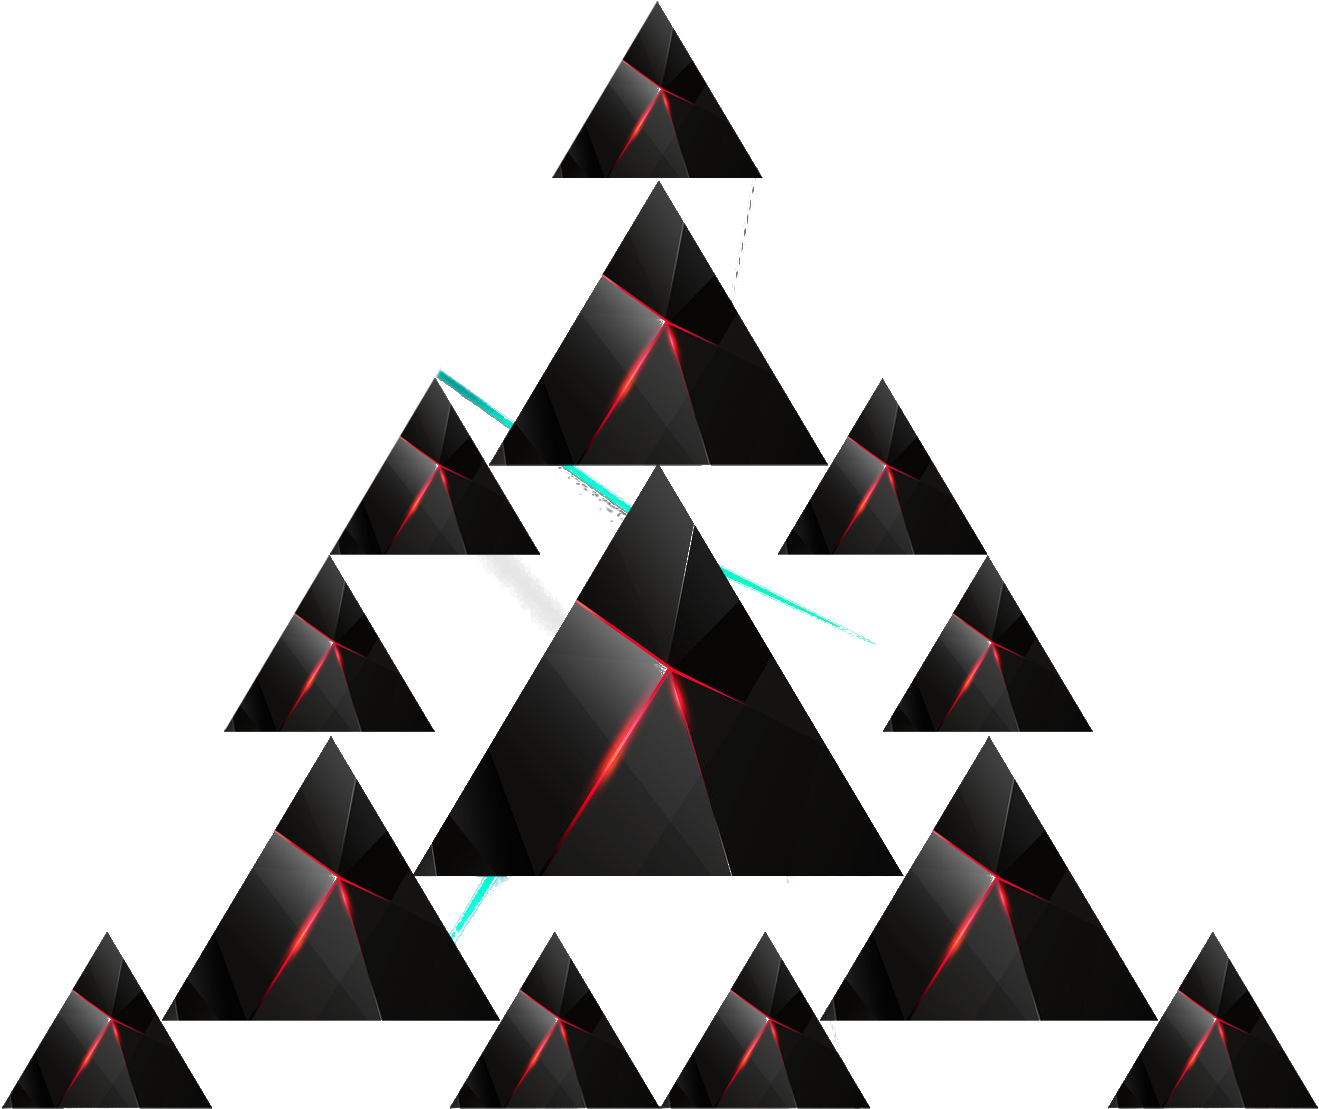
\includegraphics[width=0.5\linewidth]{img/maps/Aethereu.png}	
	
	{\textbf{Aethereu:} The space chamber is composed of multi layered triangle rooms that can rotate about one another.}
\end{center}

Spati Aethereu Thalamun (Space chamber, also sometimes referred to as just Aethereu) is the name of one of the Three Trinity Stone chambers. Specifically, This one is the space chamber. It was created by The Space Stone with remnants of the time and matter stones. Not much is known about this chamber. It is presumed to have been made when the Incantation to hide the Trinity stones was finished. The only way to reach Spati Aethereu Thalamun is to successfully travel through The Pluvian Forest. The reasons for the strange occurrences within The Pluvian Forest are believed to originate from this chamber by those who know the stories of it.

Aethereu is a trinity puzzle. There are many ways to navigate it but only one successful. Wrong navigations will lead to negative consequences. Each stone has an effect on the chamber which needs to be navigated simultaneously. If one, or two of three are done successfully but not the third, this is when a negative consequence happens.

First, the chamber consists of 13 triangular rooms. It can be represented by a hexagonal diagram like the one below.

\begin{center}
	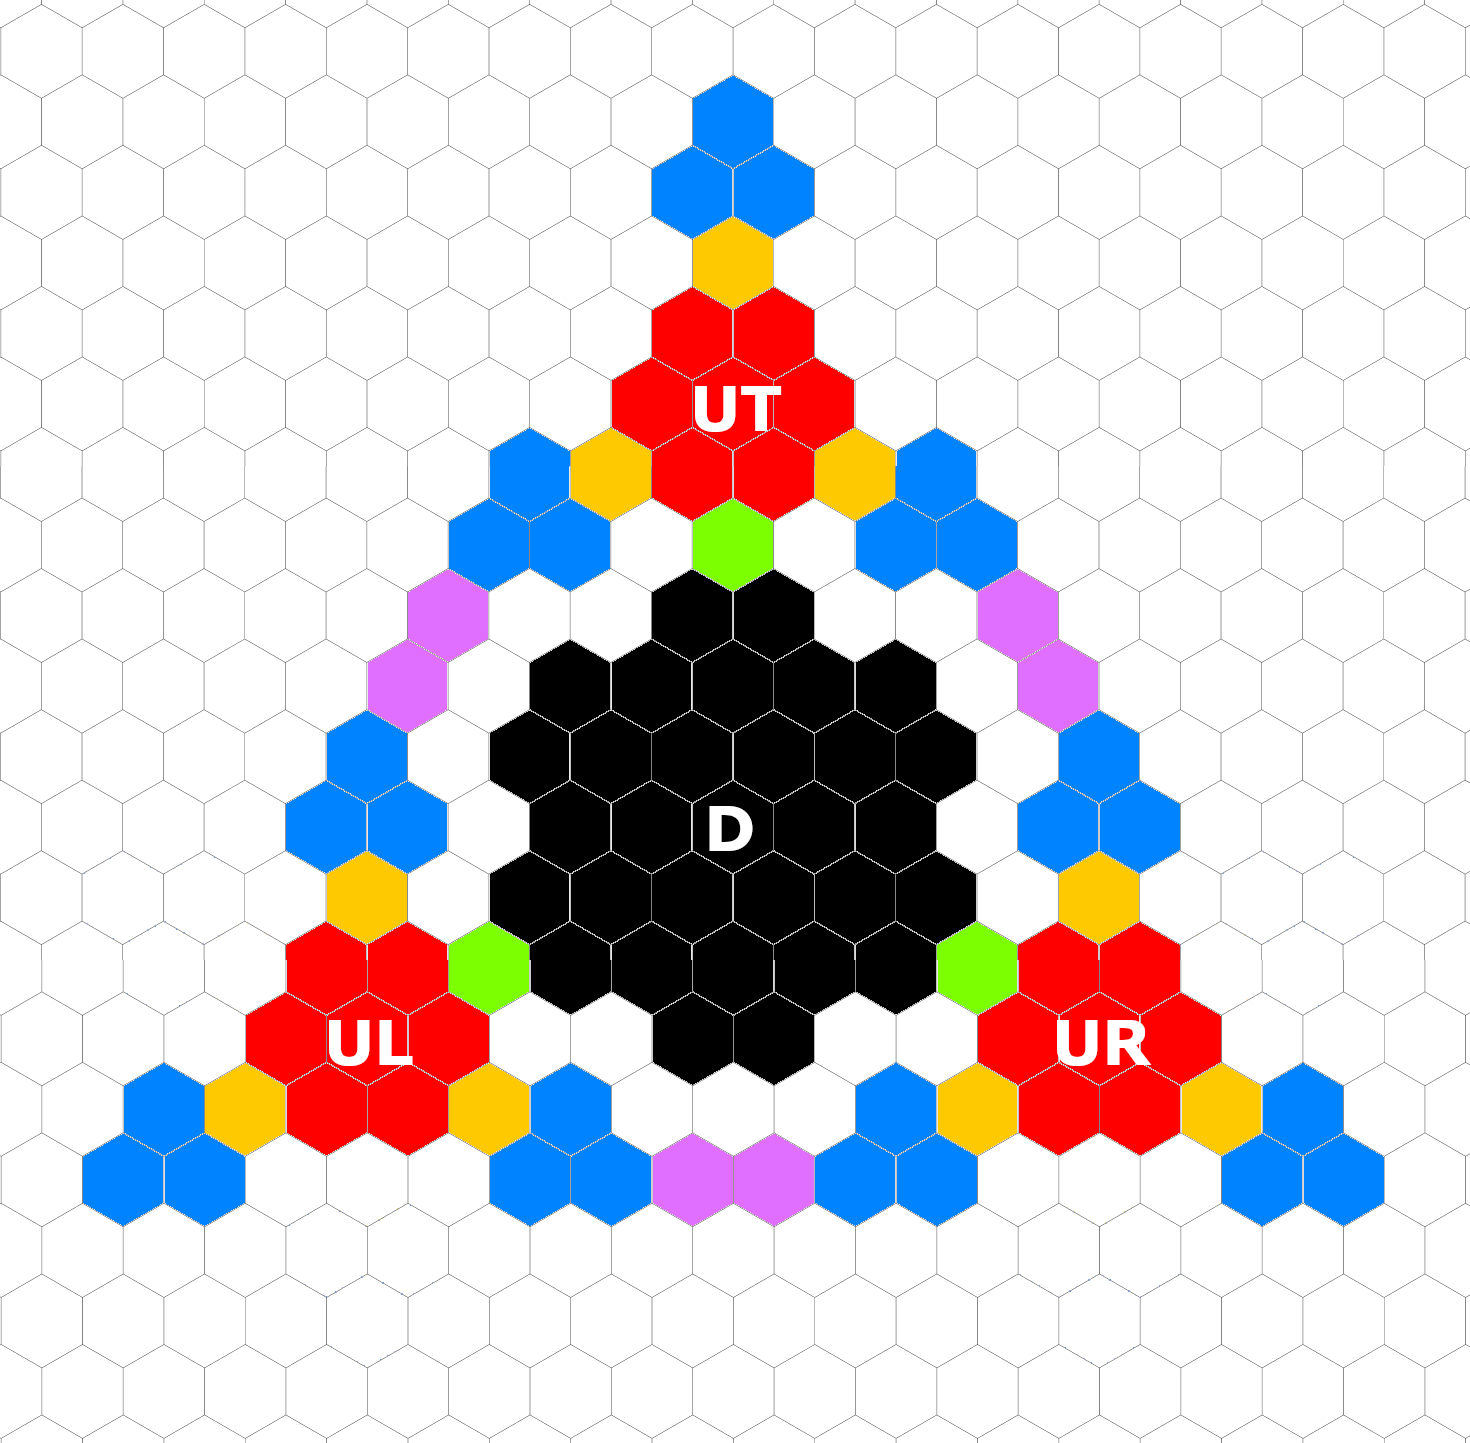
\includegraphics[width=0.5\linewidth]{img/Aethereu/U.png}
\end{center}

The black, red, and blue colors represent rooms. Black is the main chamber, red are slightly smaller chambers, and blue are small rooms. The rooms are designed such that they can rotate about one another. The red rooms can rotate around the black, and the blue can rotate around the red. The orange and purple colors represent connections between the rooms (where doorways would appear). The rooms rotate when exited and the label in a room exited represents the rotation that is undergone. This rotation is instant and any doorways would disappear and reappear in new locations if necessary. The DM can choose whether to have them rotate when te entire party is entering or just one player based on the situation. The rotation is always clockwise. The possible configurations are as follows.

\begin{center}
	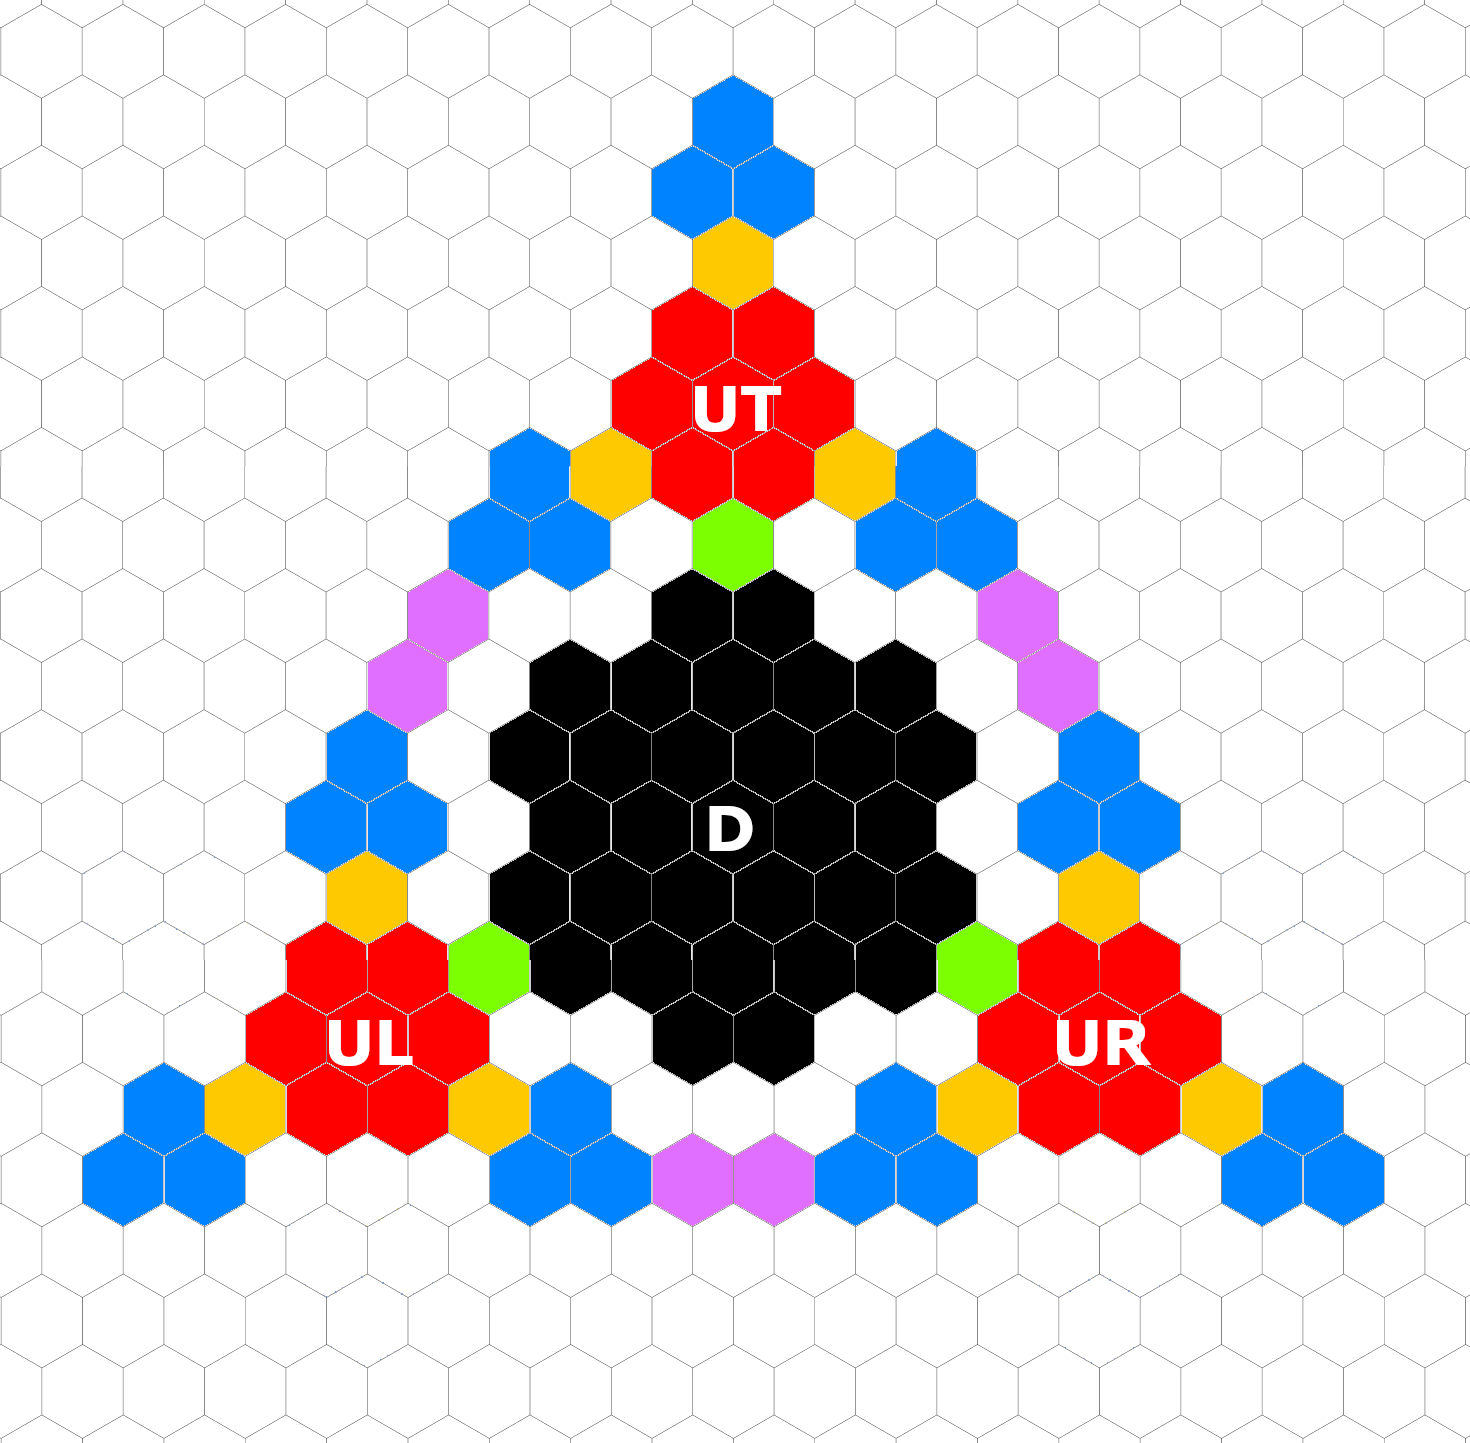
\includegraphics[width=0.45\linewidth]{img/Aethereu/U.png}
	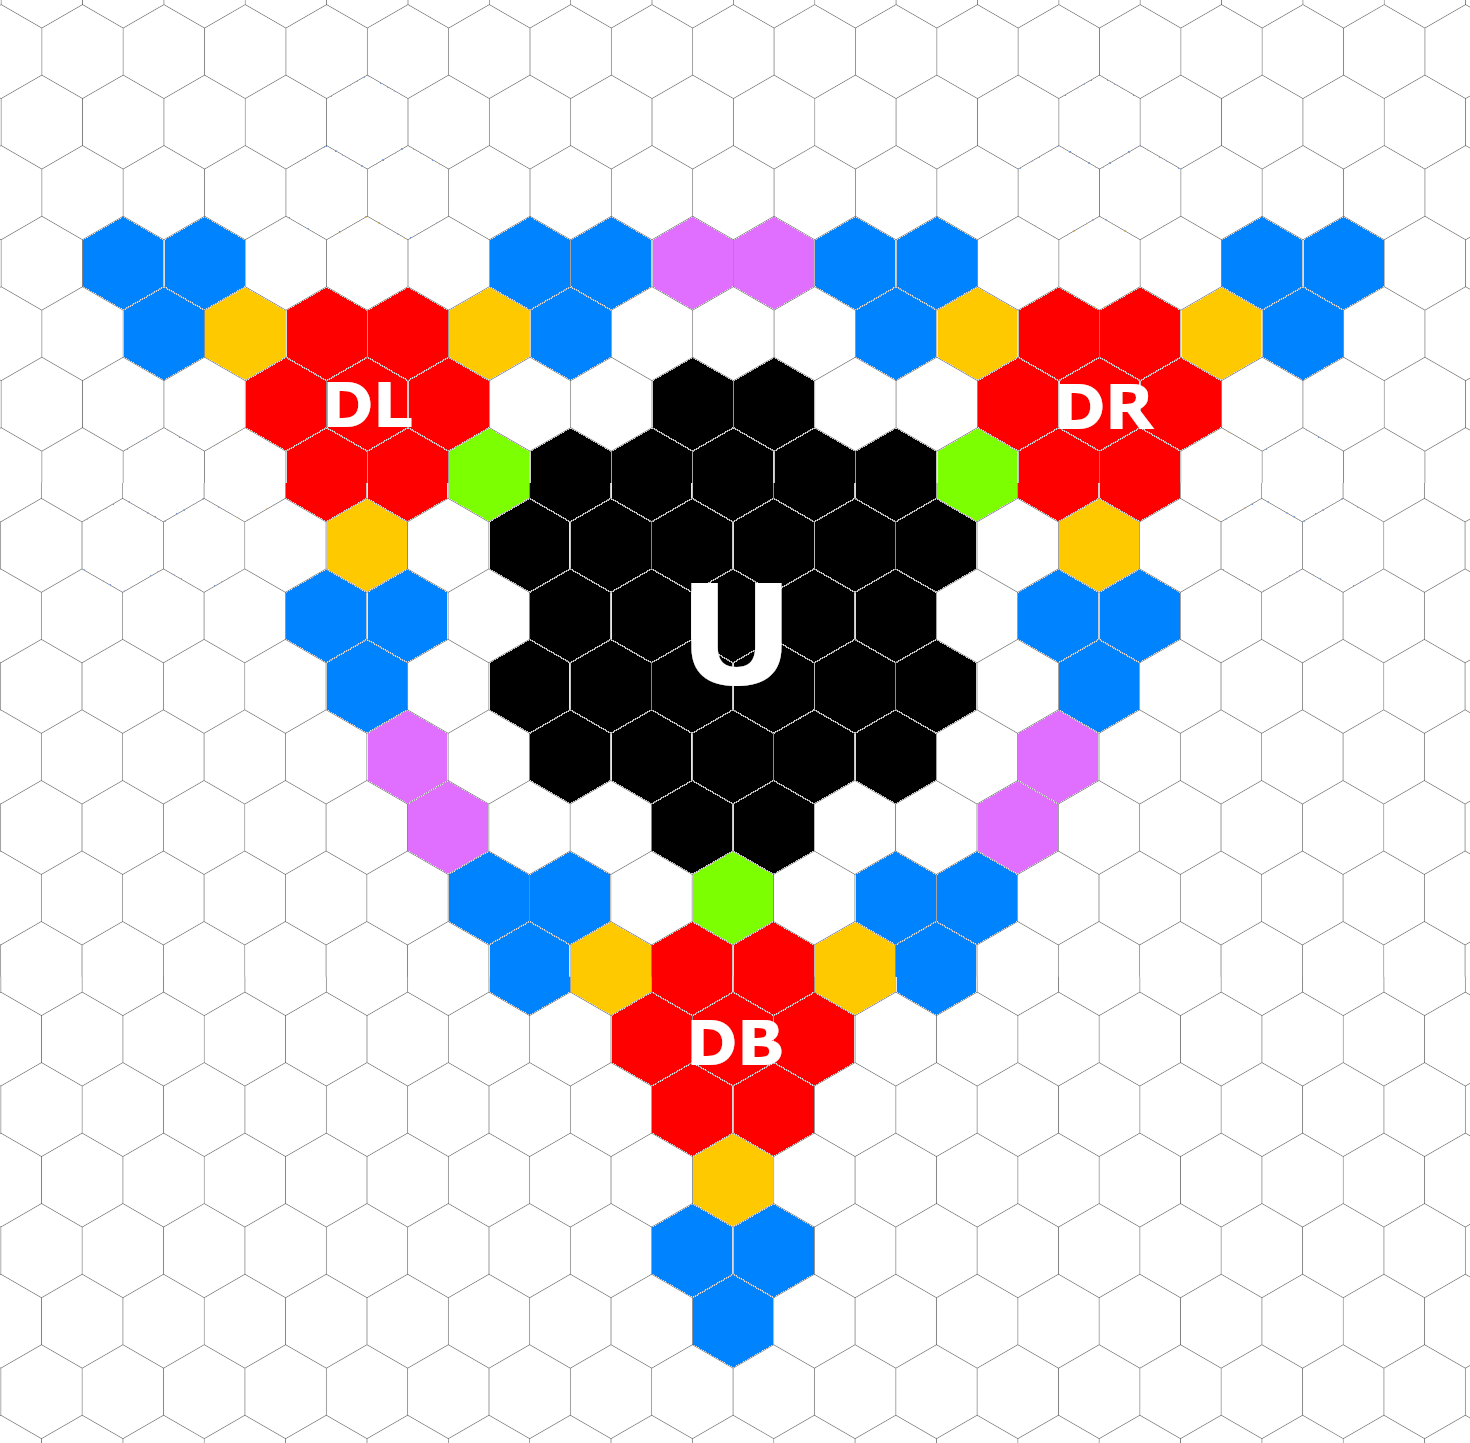
\includegraphics[width=0.45\linewidth]{img/Aethereu/D.png}
	
	\textbf{U} \hspace{7.5cm} \textbf{D}
	
	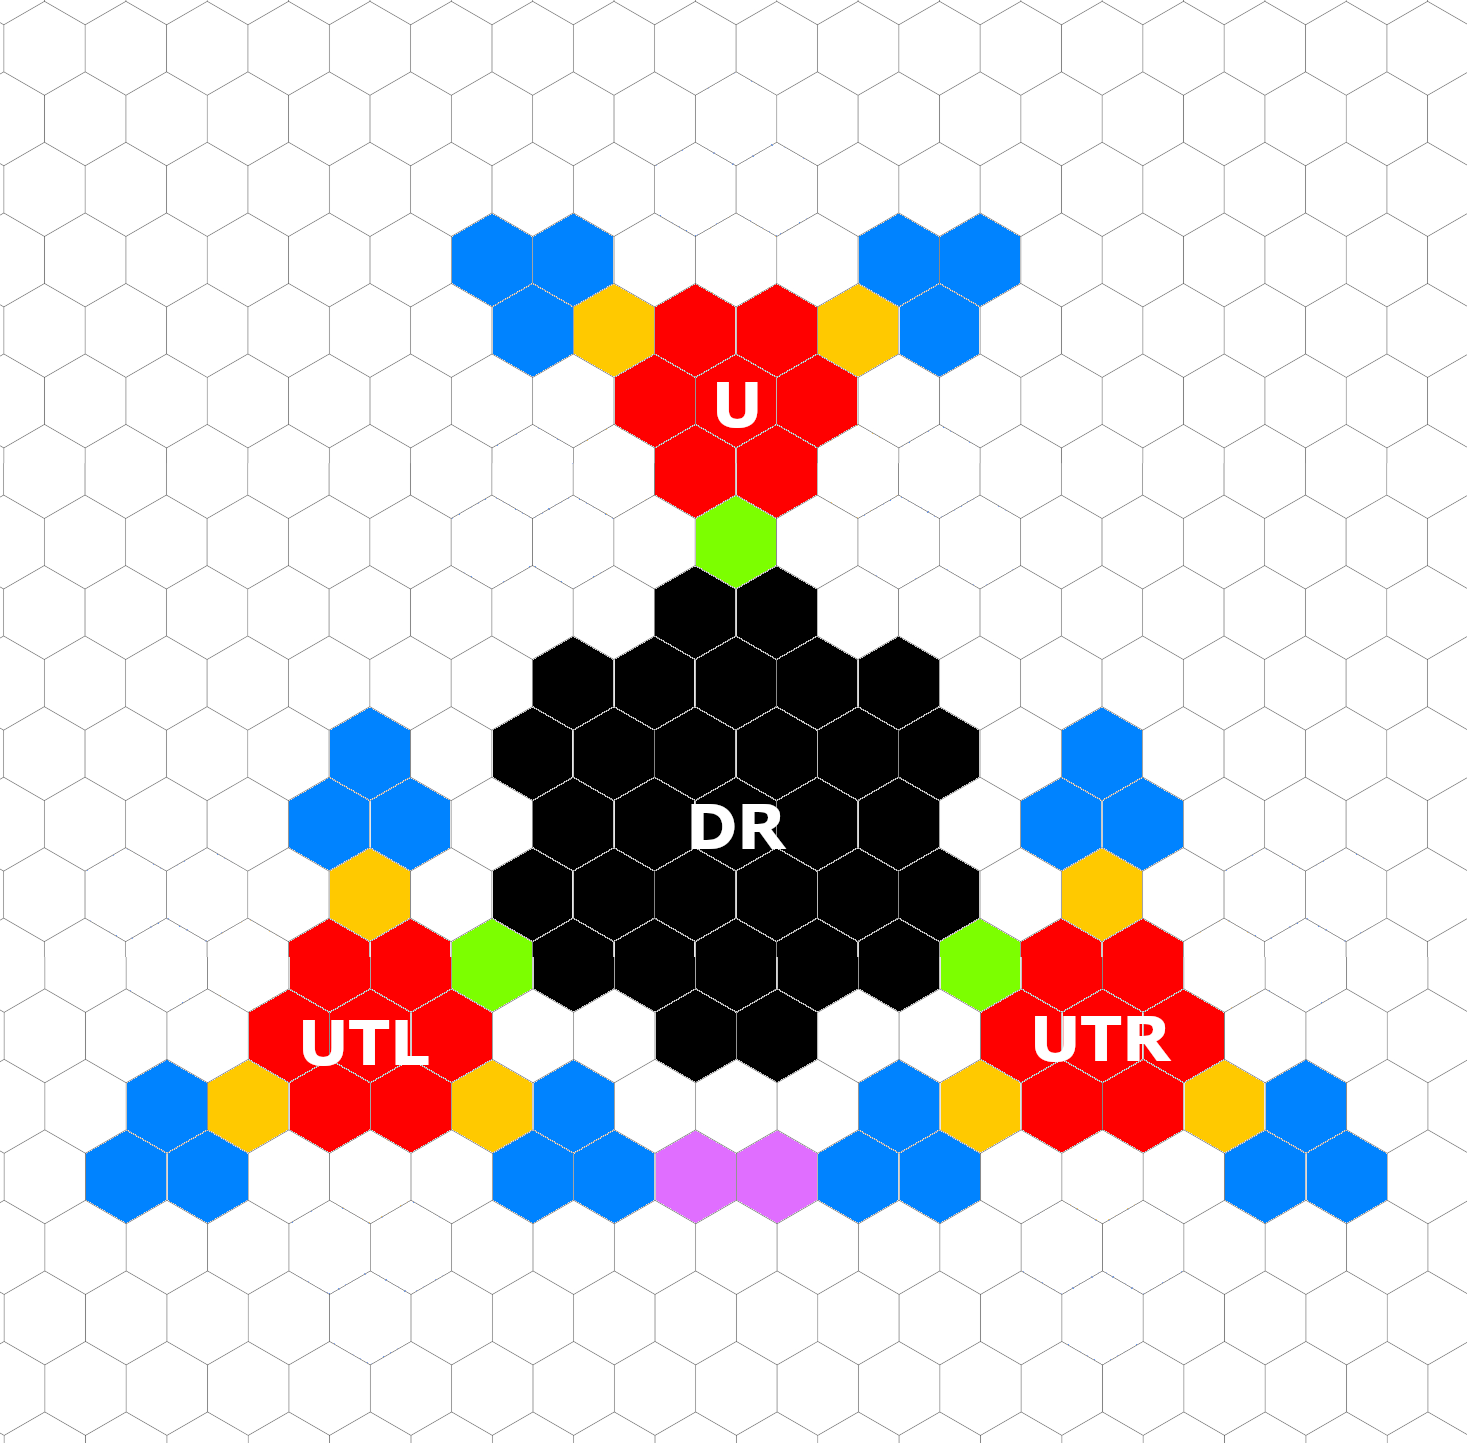
\includegraphics[width=0.45\linewidth]{img/Aethereu/UT.png}
	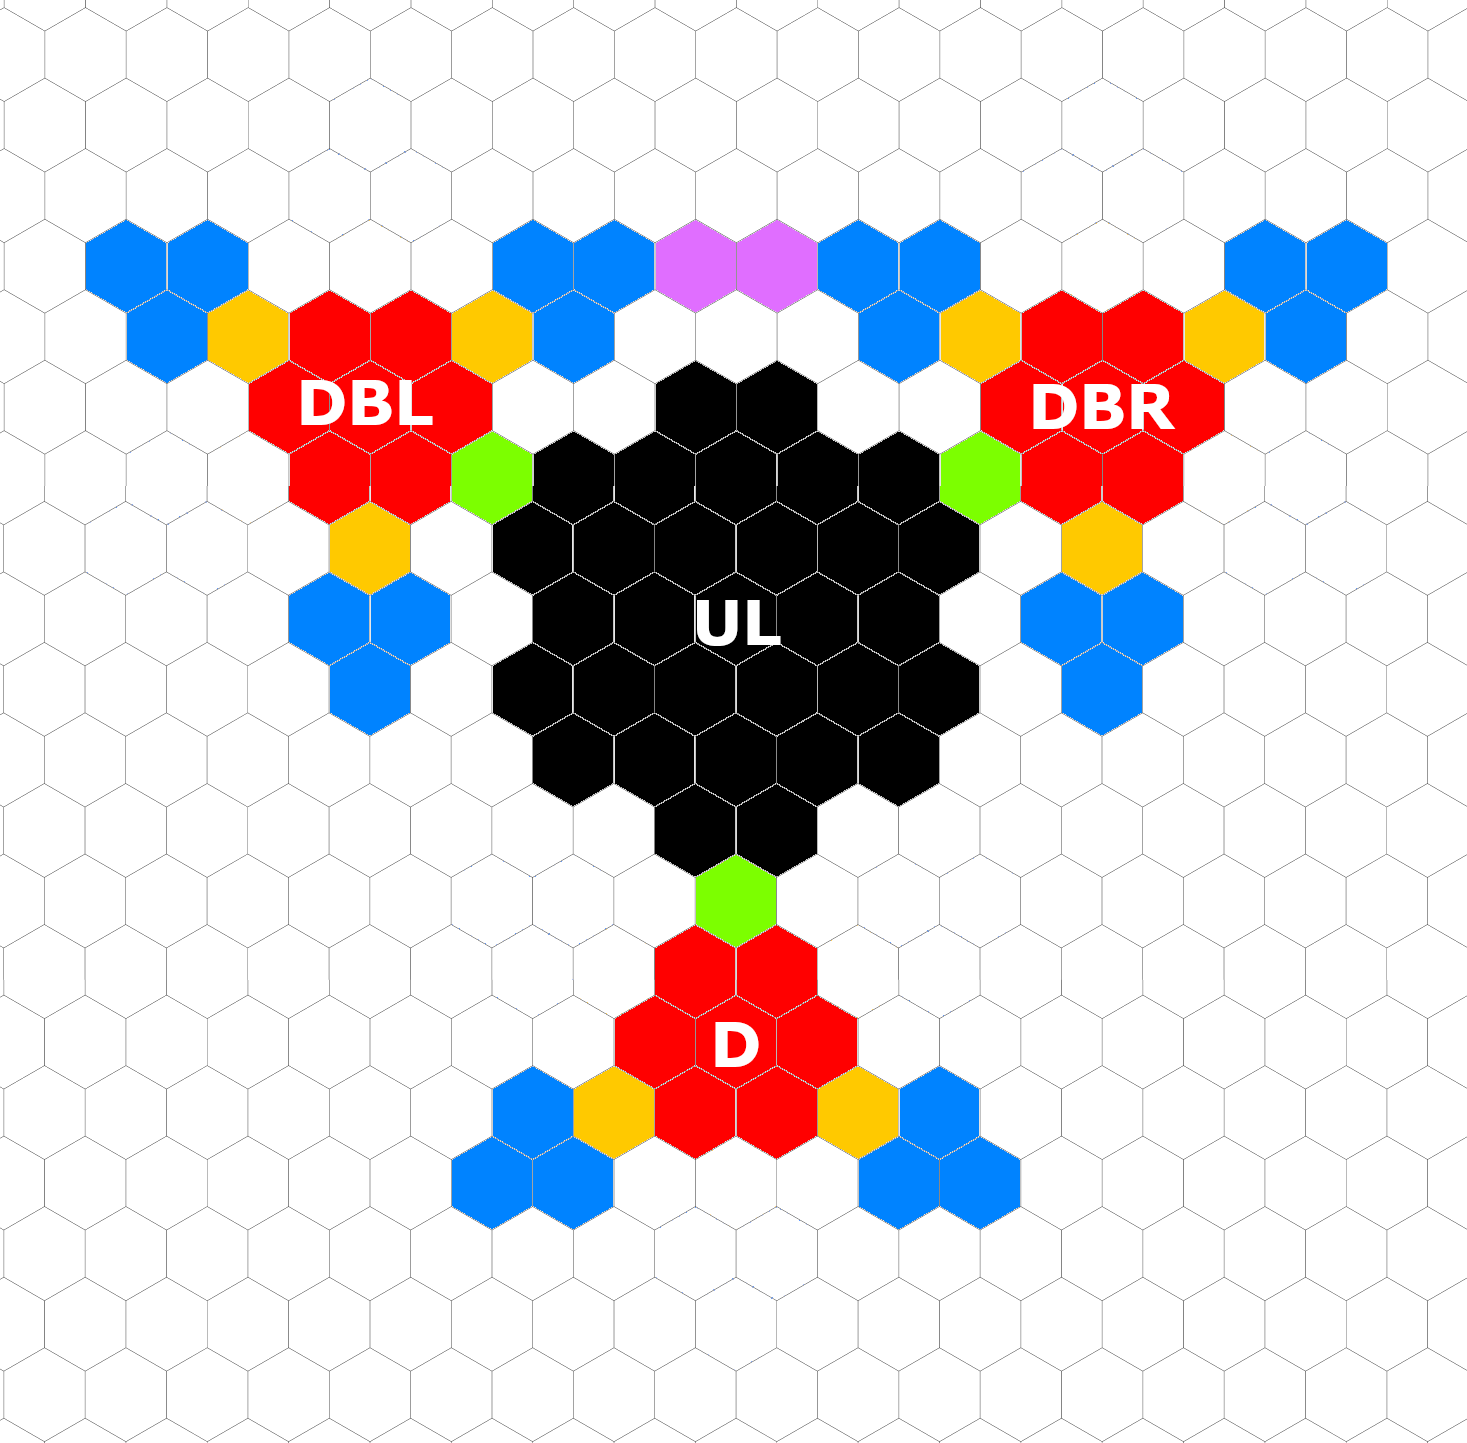
\includegraphics[width=0.45\linewidth]{img/Aethereu/DB.png}
	
	\textbf{UT} \hspace{7.3cm} \textbf{DB}
	
	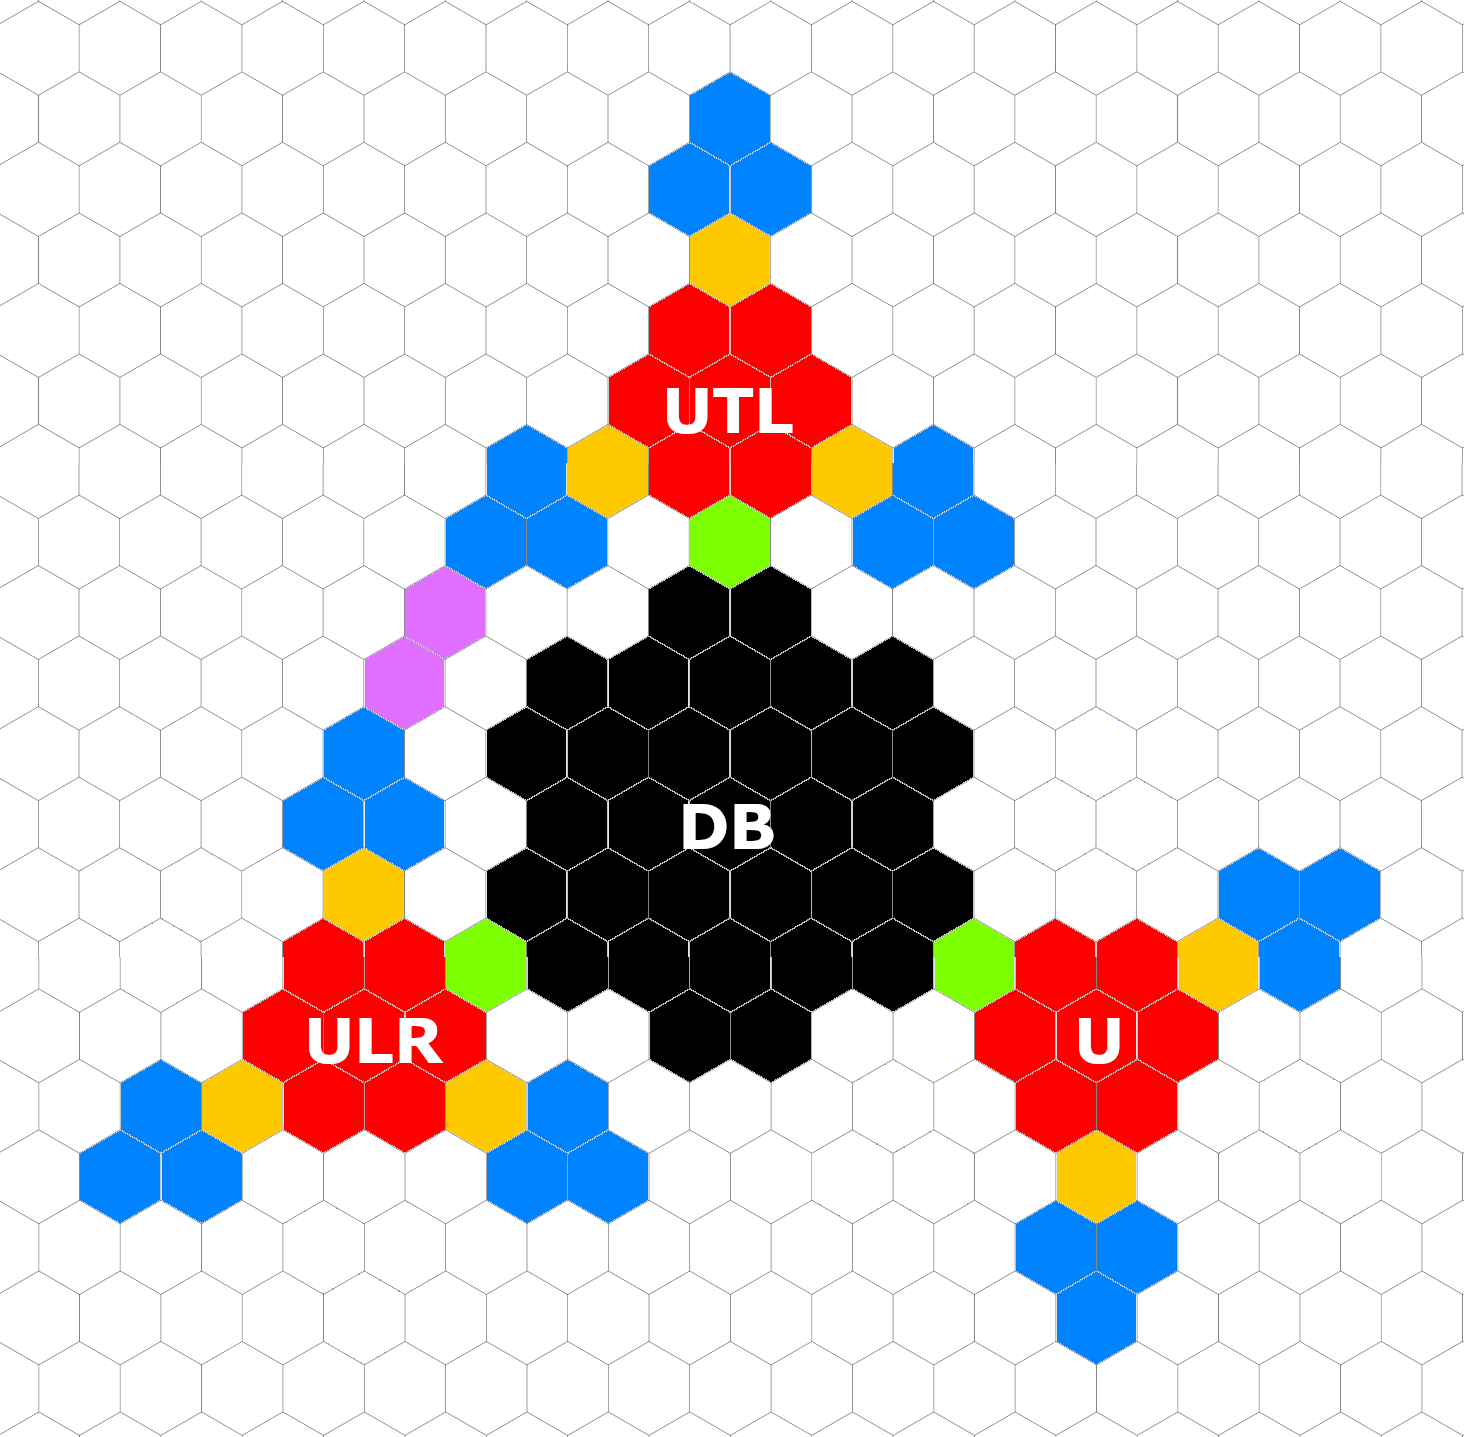
\includegraphics[width=0.45\linewidth]{img/Aethereu/UR.png}
	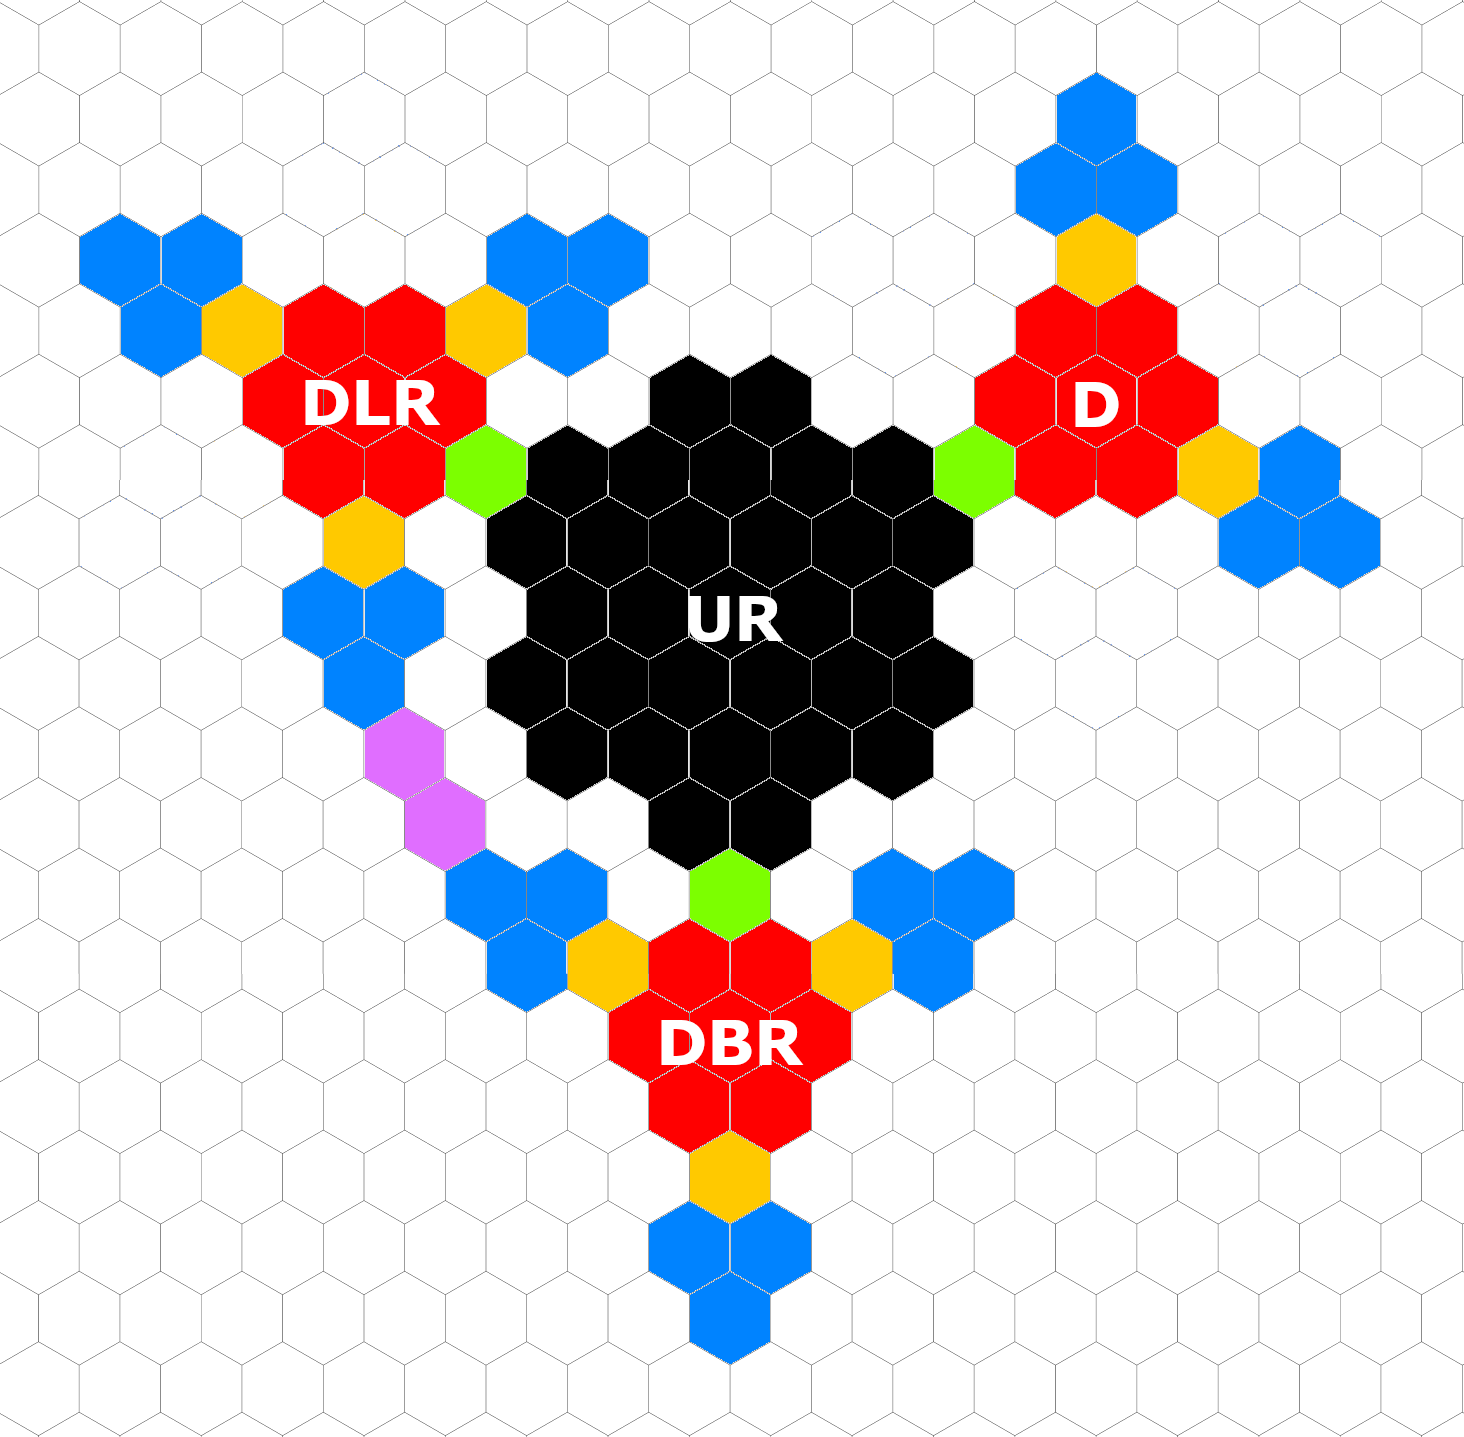
\includegraphics[width=0.45\linewidth]{img/Aethereu/DR.png}
		
	\textbf{UR} \hspace{7.3cm} \textbf{DR}
	
	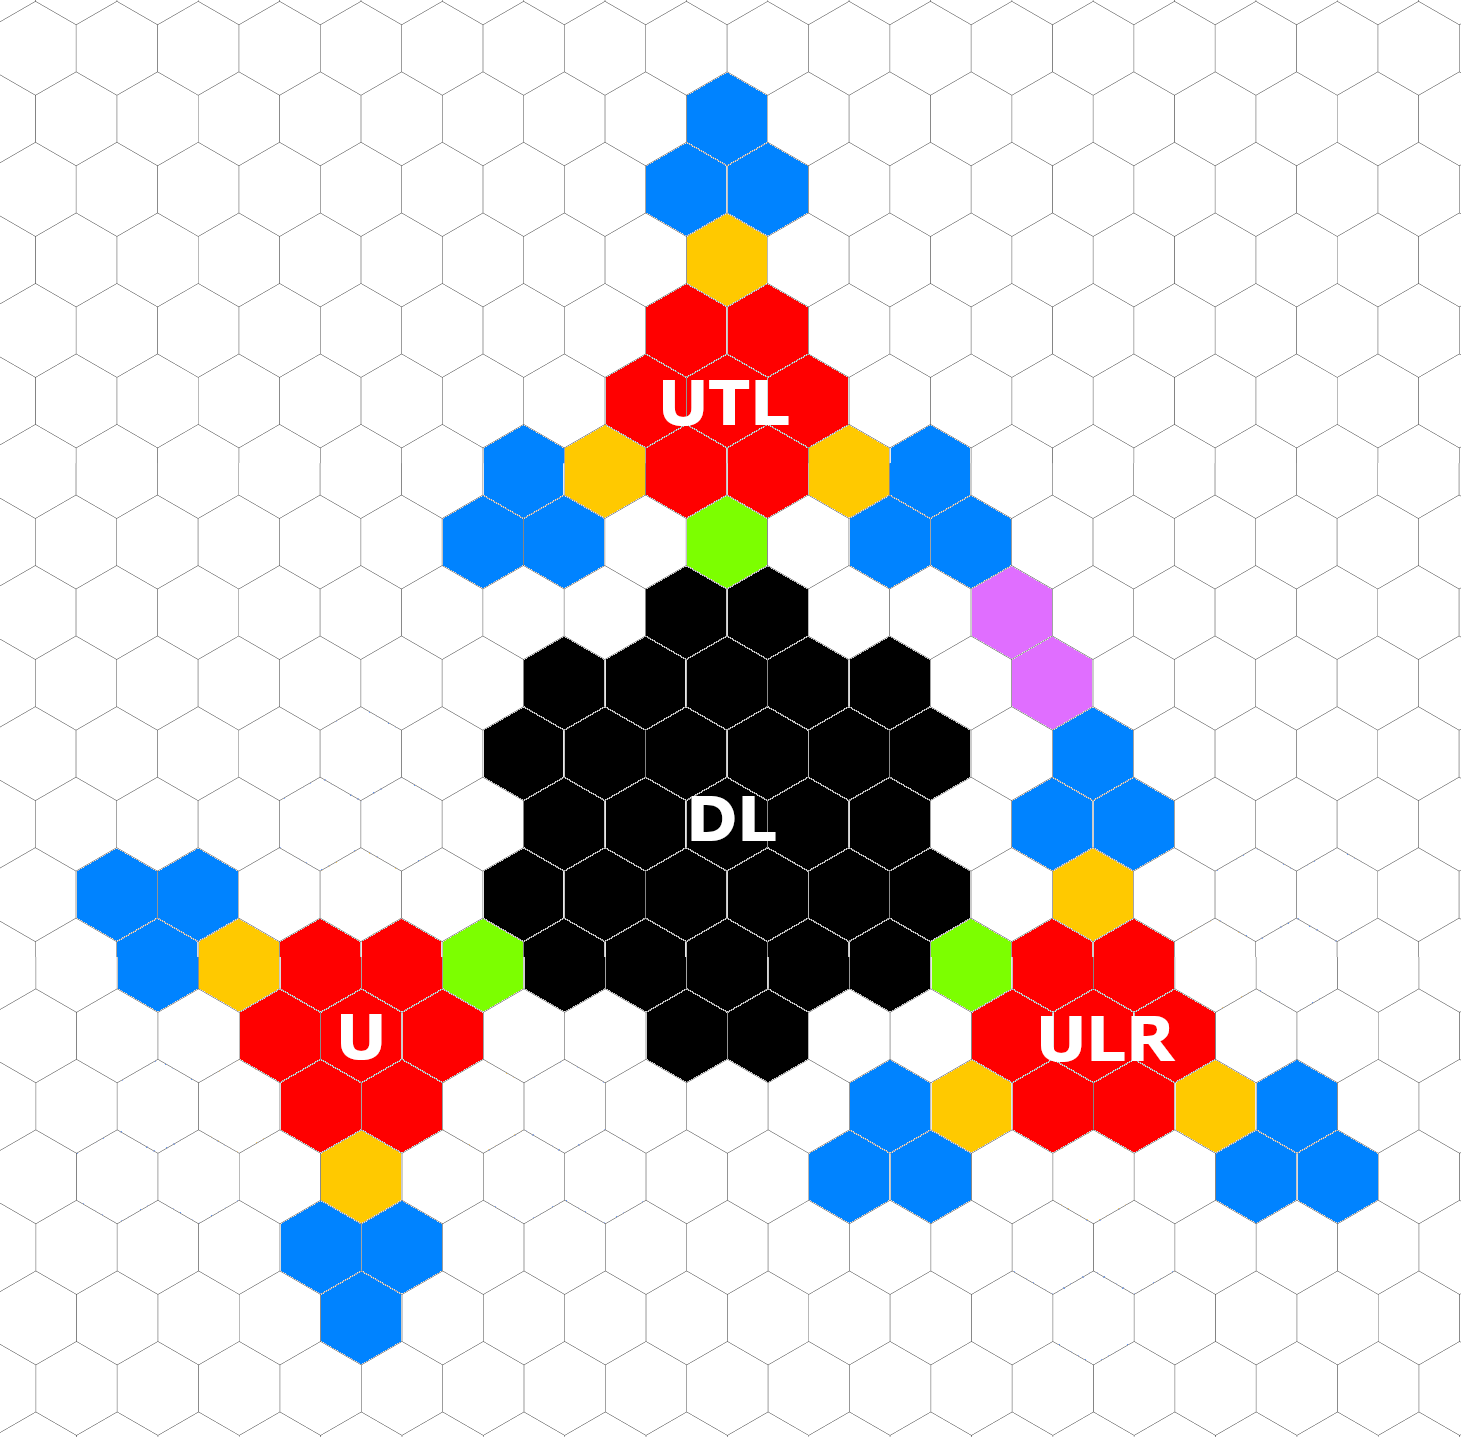
\includegraphics[width=0.45\linewidth]{img/Aethereu/UL.png}
	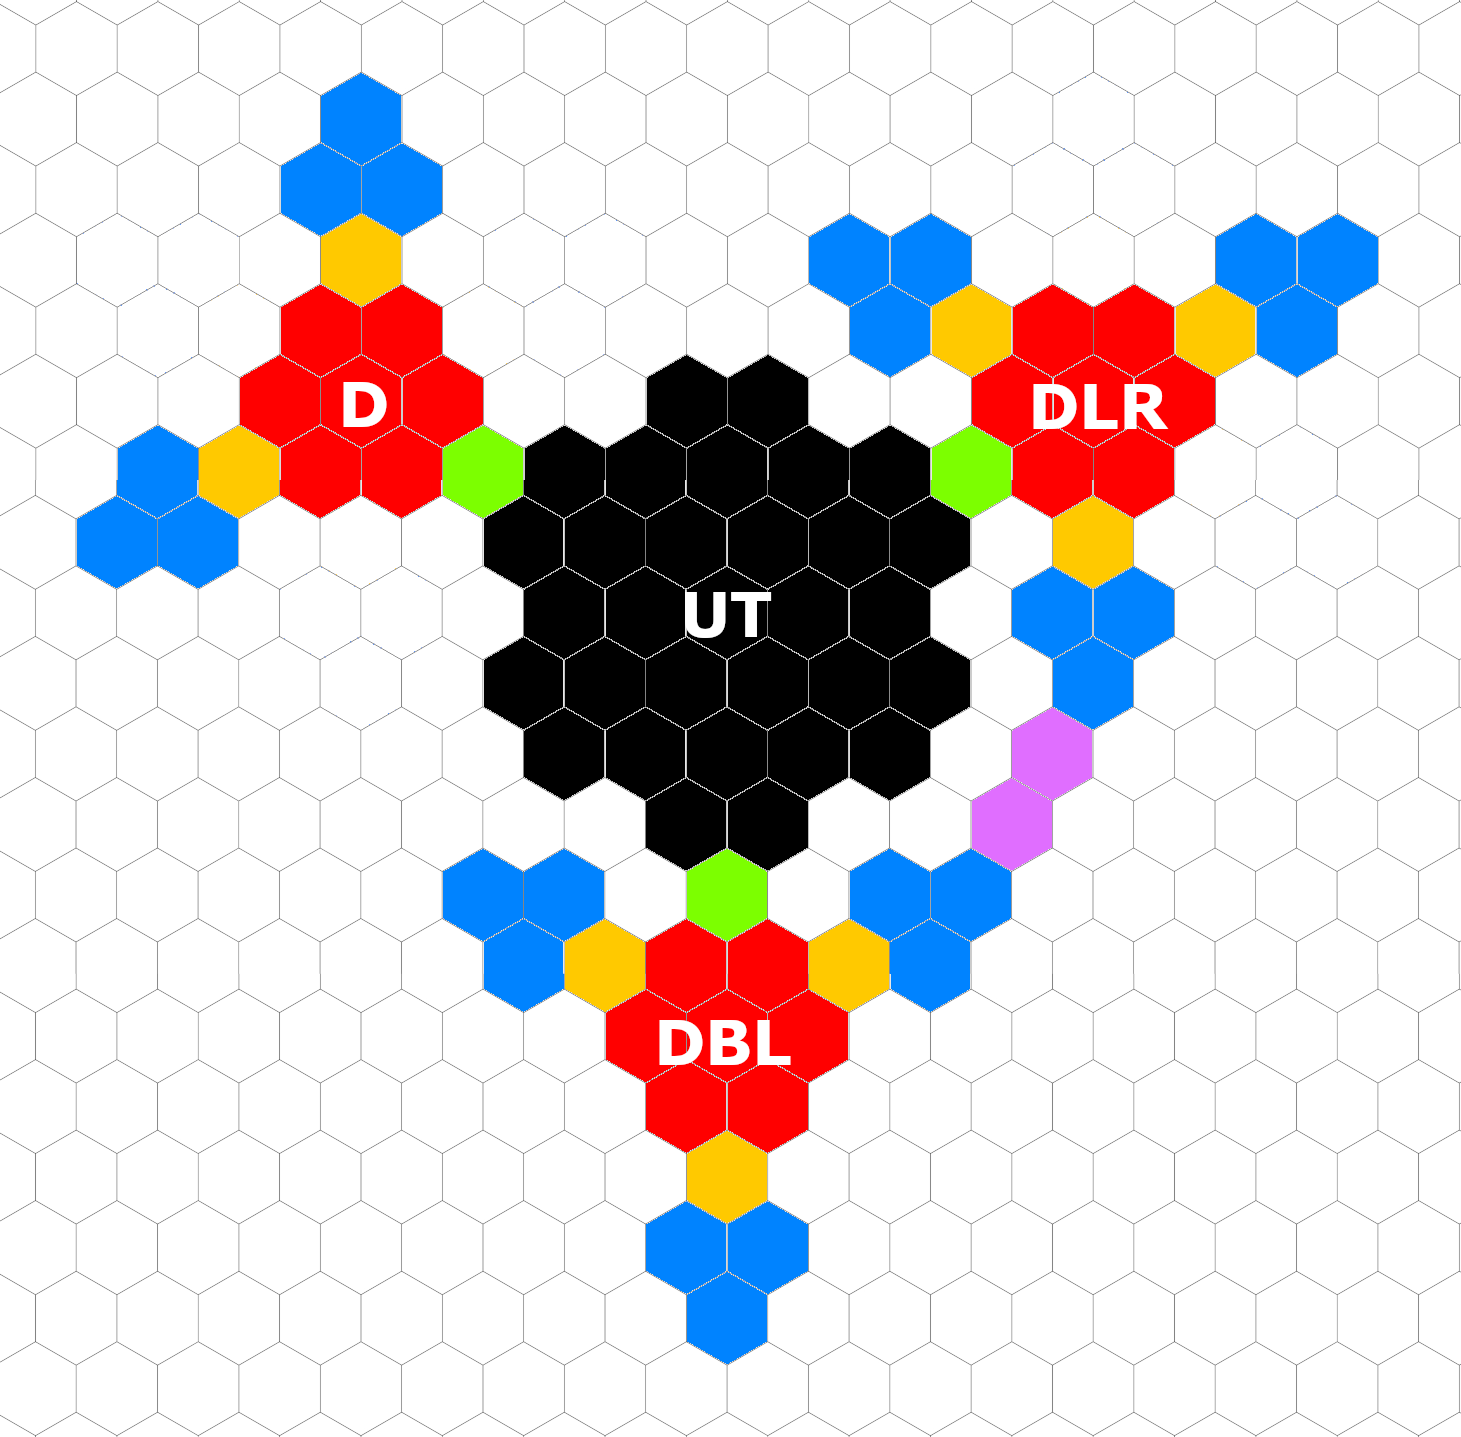
\includegraphics[width=0.45\linewidth]{img/Aethereu/DL.png}
		
	\textbf{UL} \hspace{7.3cm} \textbf{DL}
	
	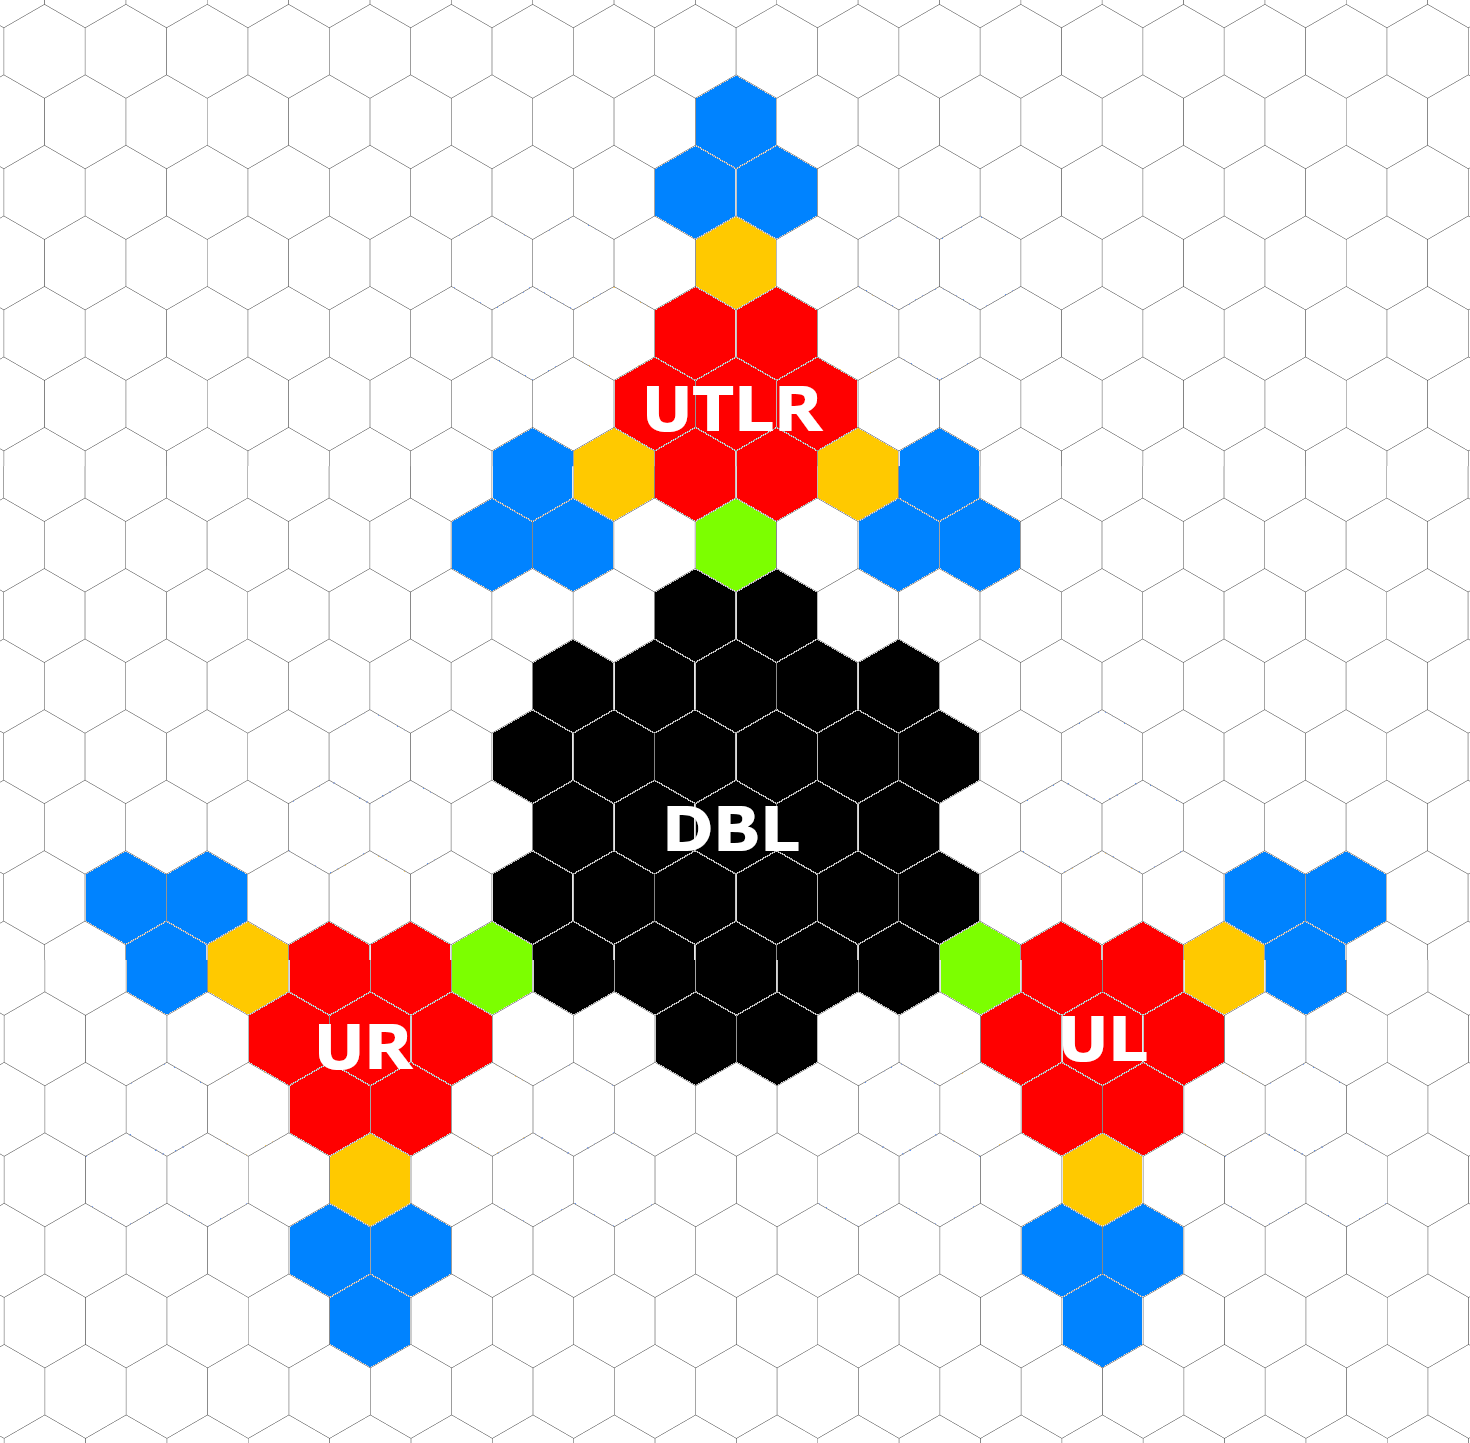
\includegraphics[width=0.45\linewidth]{img/Aethereu/ULR.png}
	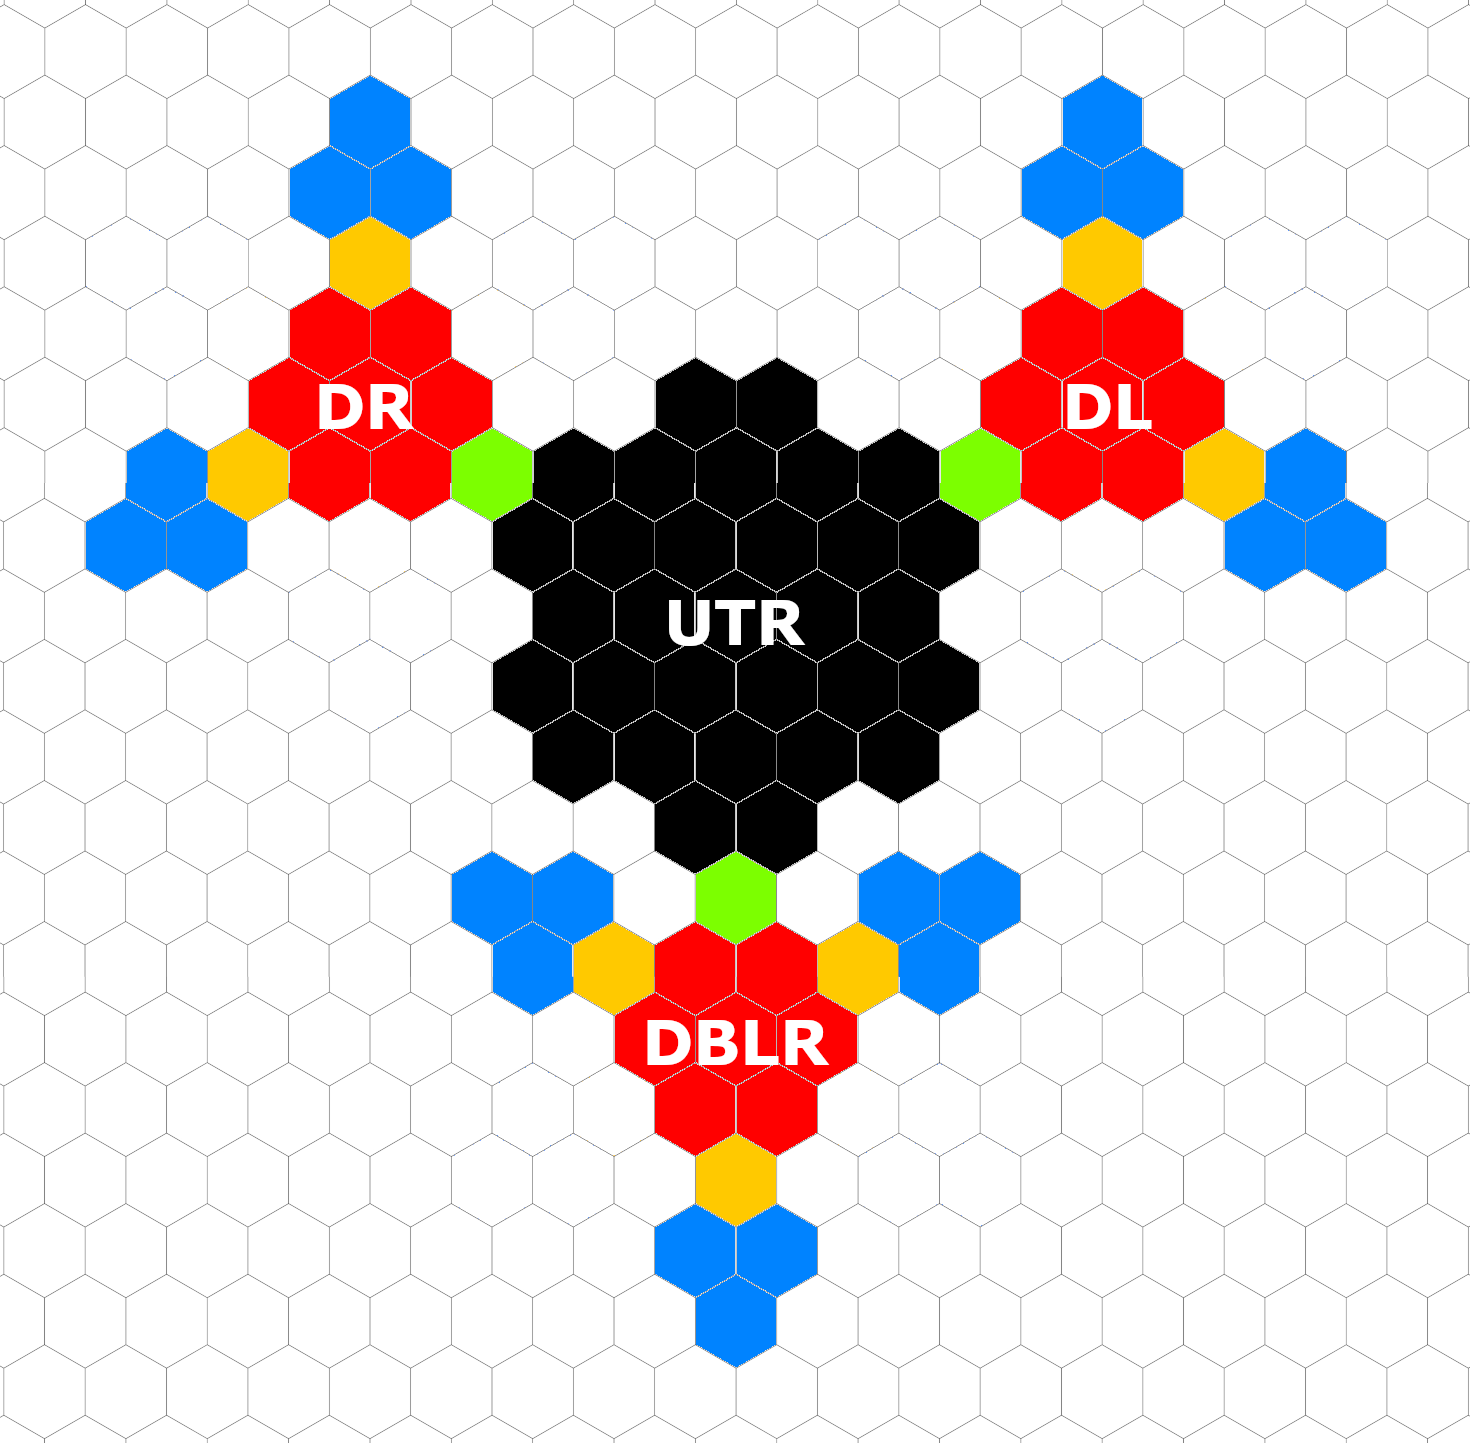
\includegraphics[width=0.45\linewidth]{img/Aethereu/DLR.png}
		
	\textbf{UTR} \hspace{7cm} \textbf{DBR}
	
	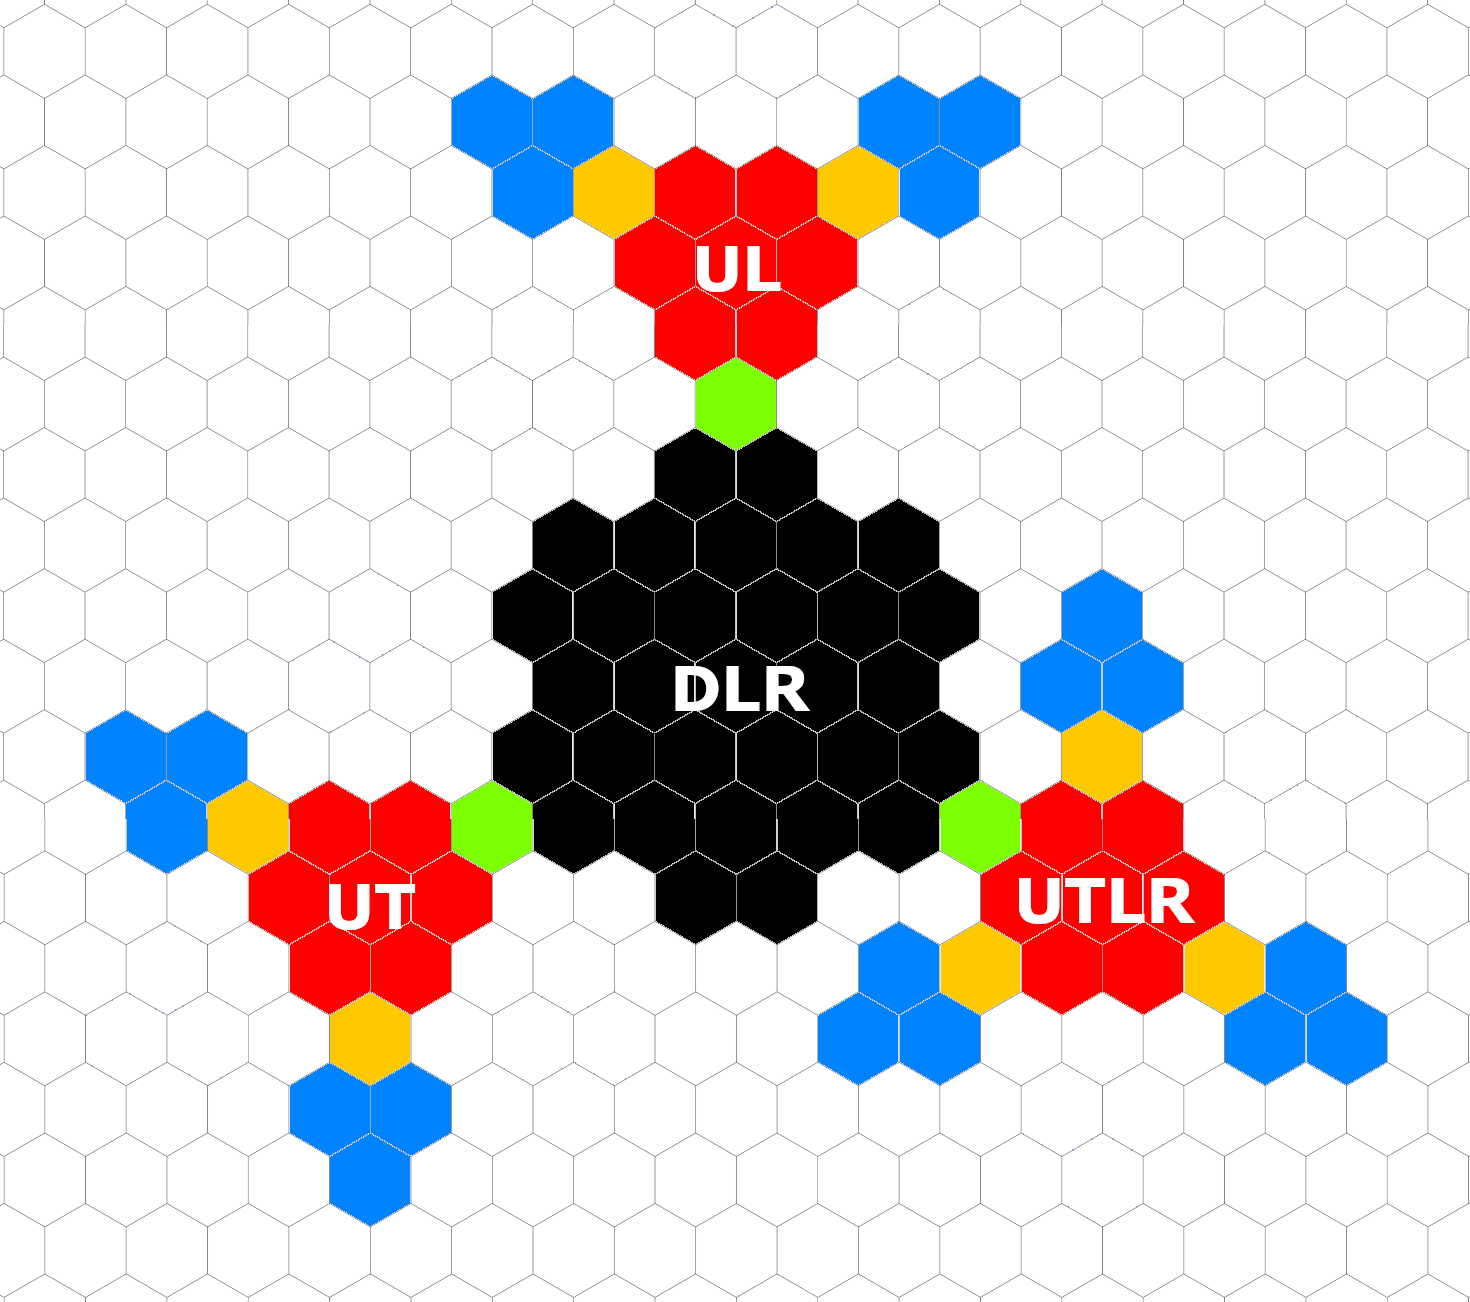
\includegraphics[width=0.45\linewidth]{img/Aethereu/UTL.png}
	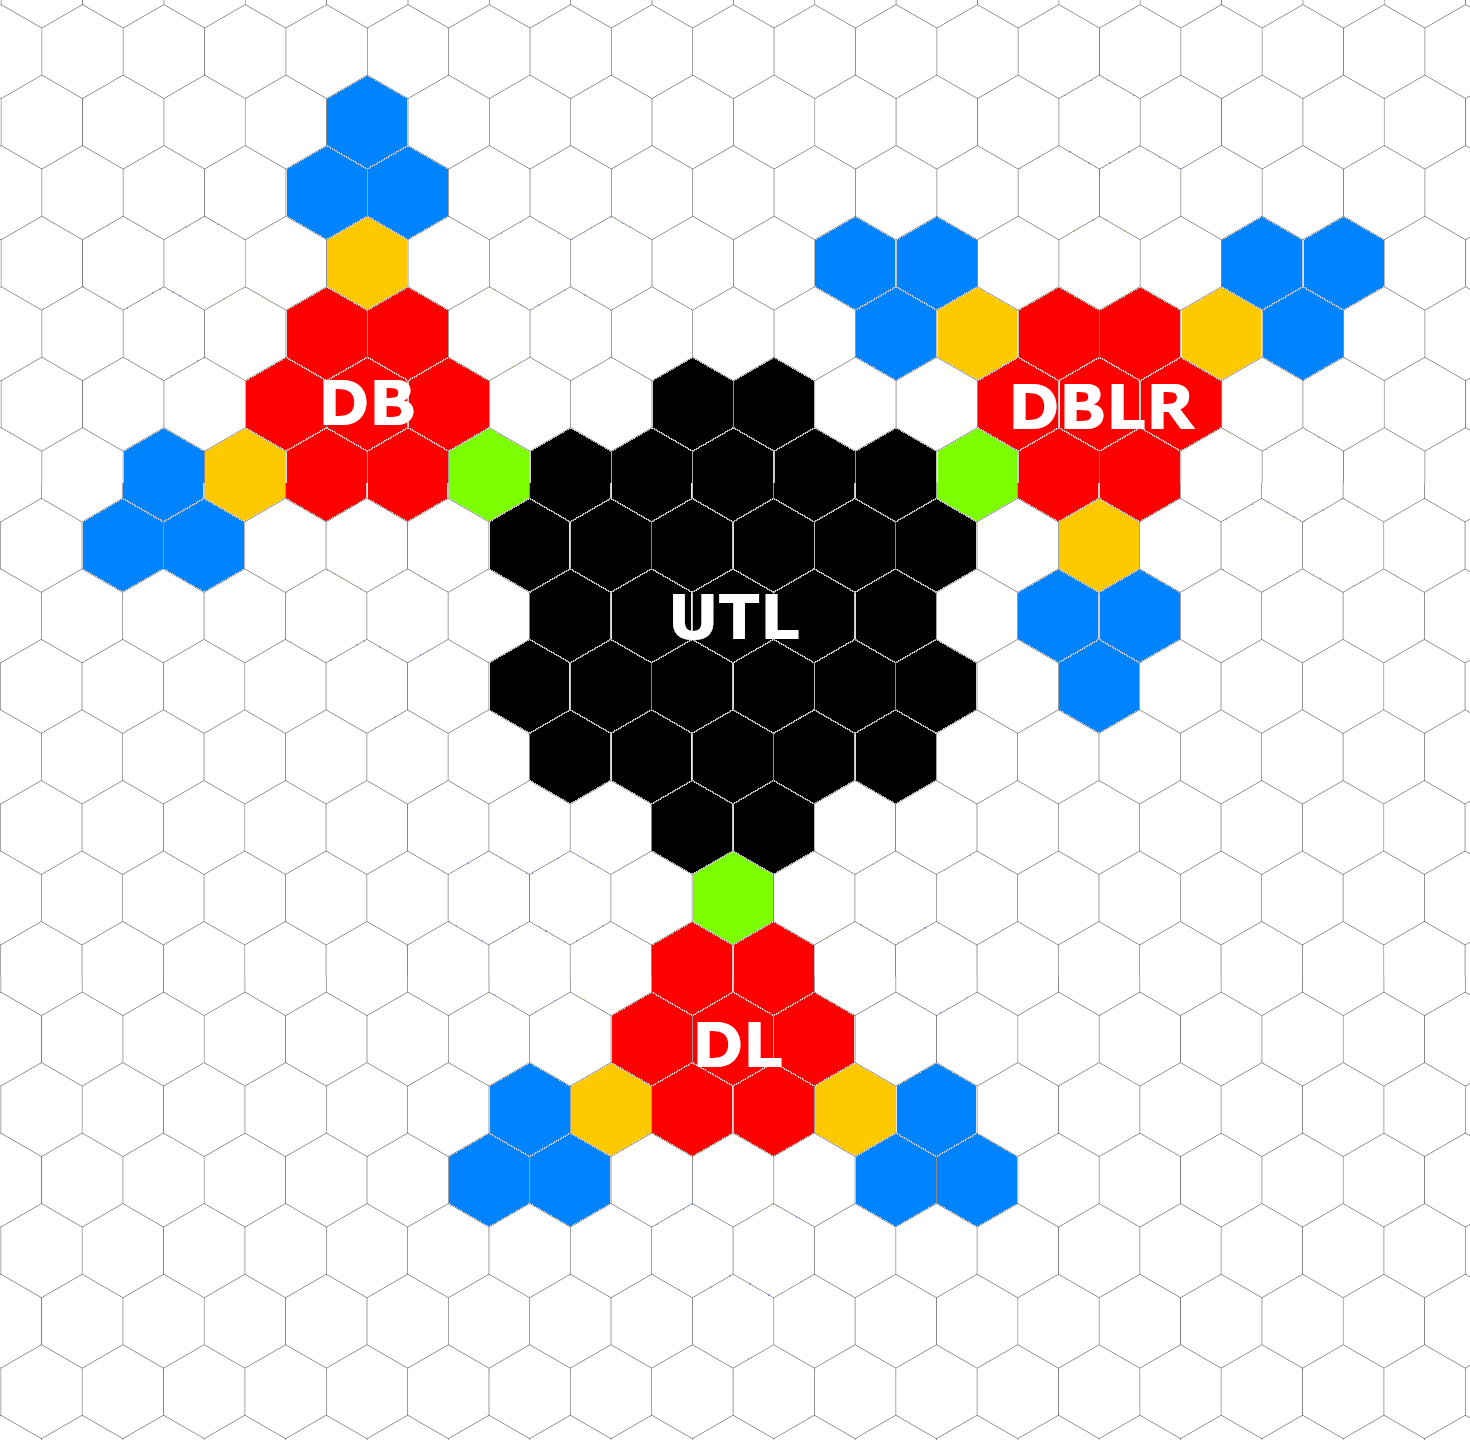
\includegraphics[width=0.45\linewidth]{img/Aethereu/DBL.png}
		
	\textbf{UTL} \hspace{7cm} \textbf{DBL}
	
	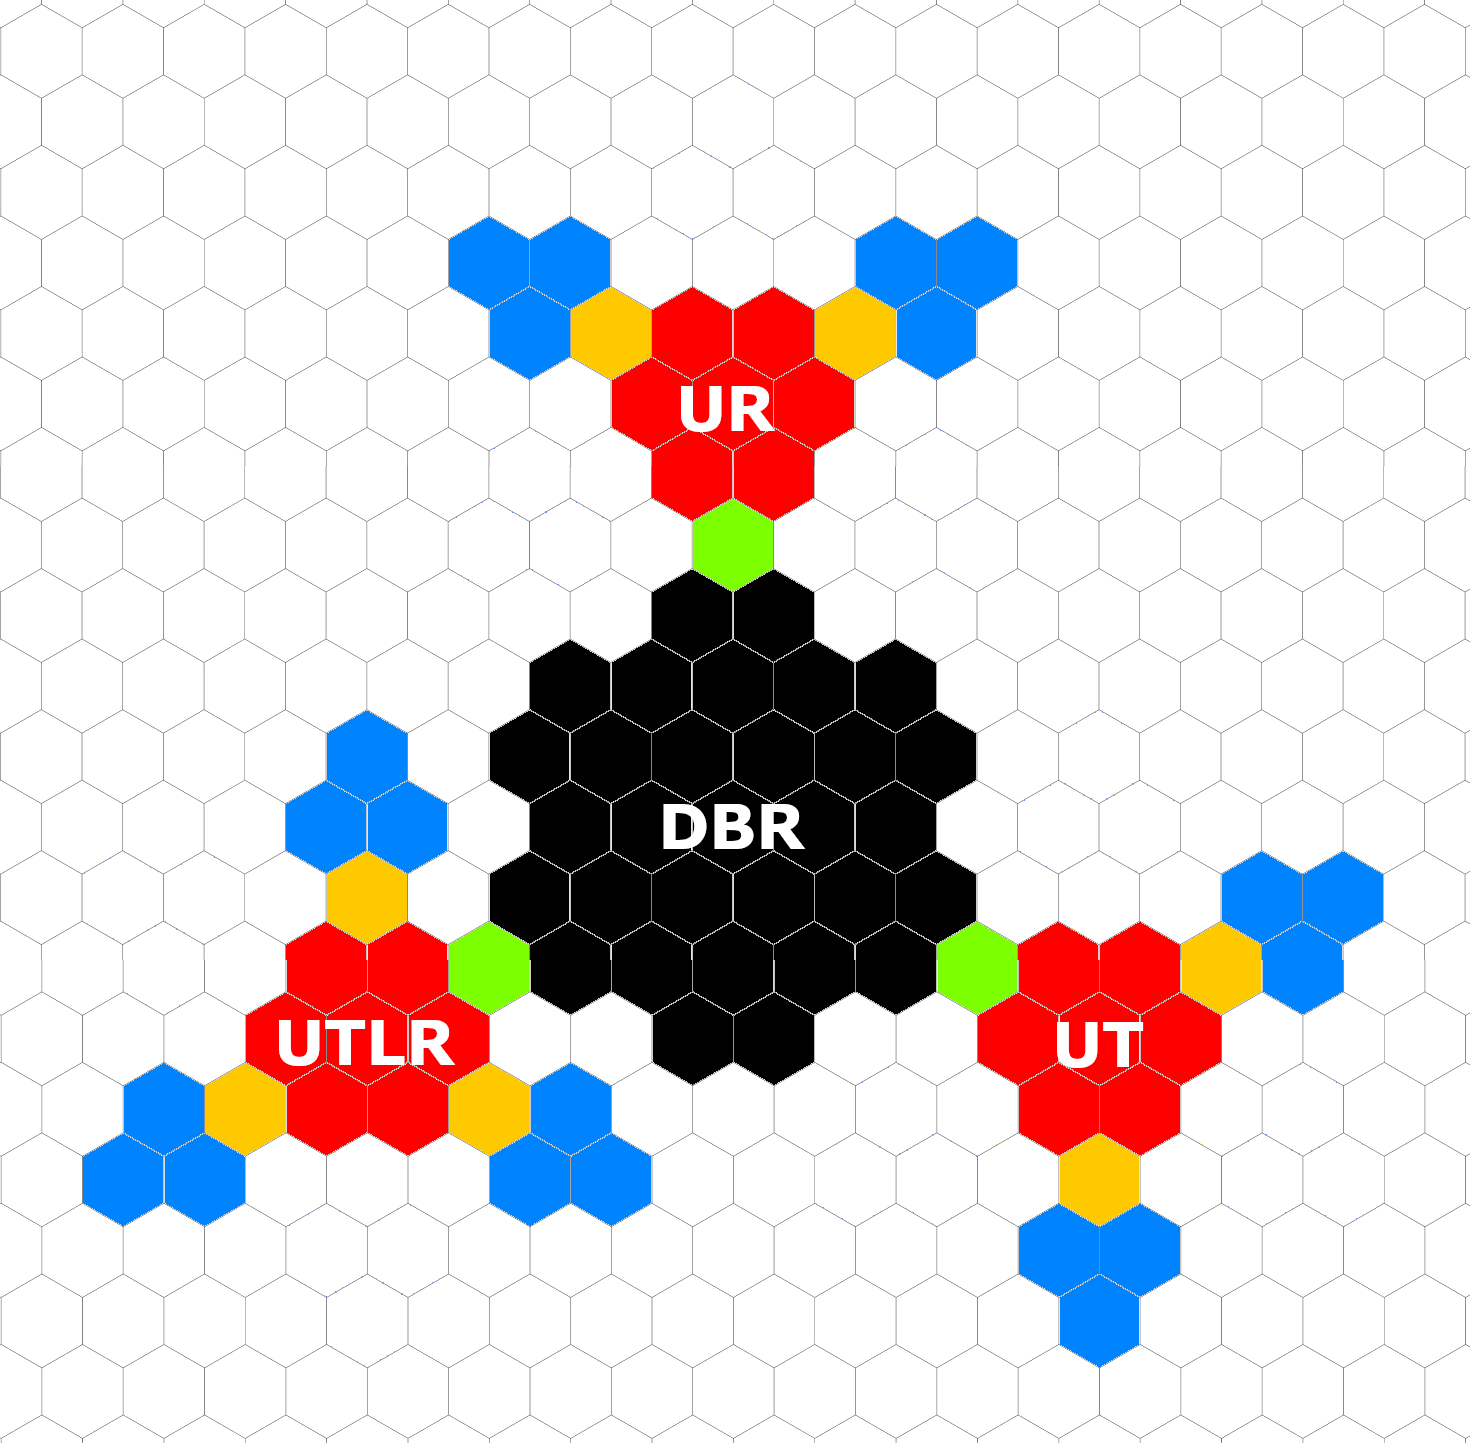
\includegraphics[width=0.45\linewidth]{img/Aethereu/UTR.png}
	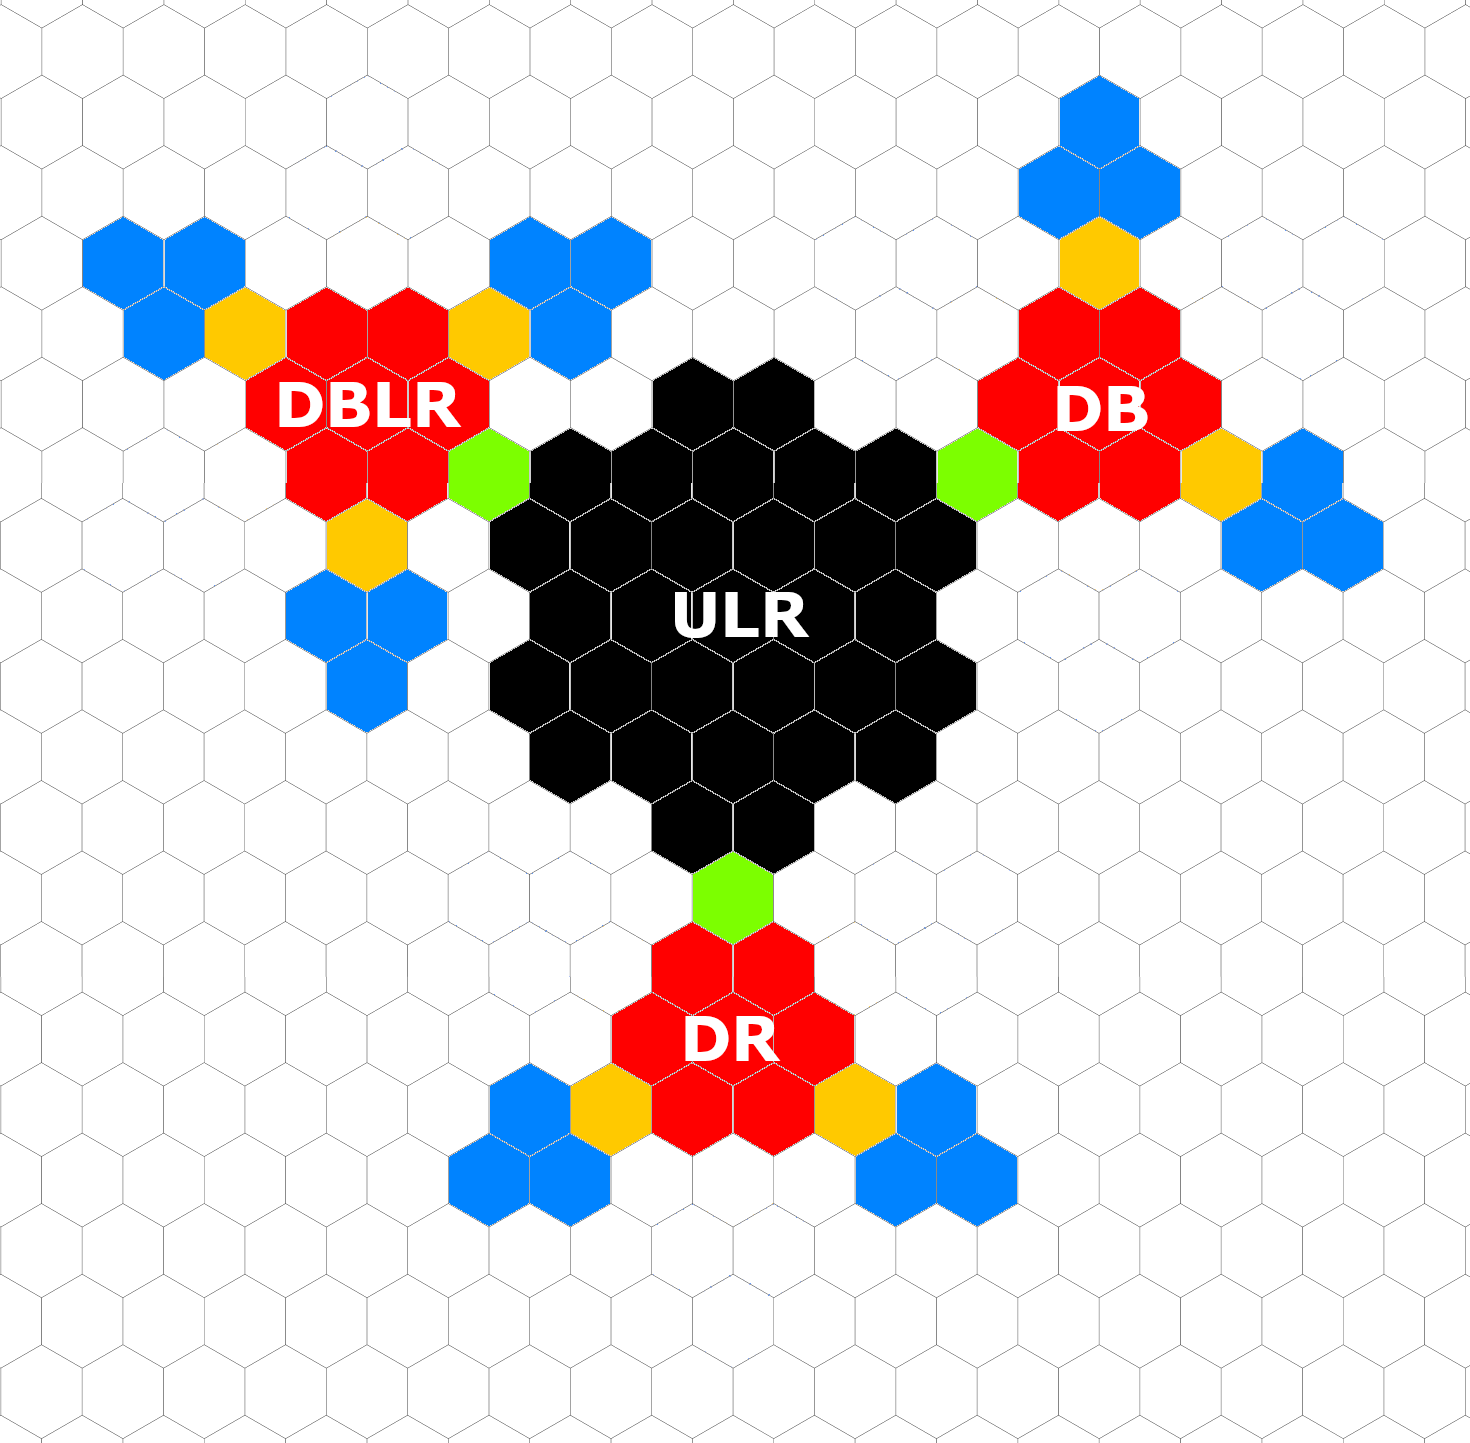
\includegraphics[width=0.45\linewidth]{img/Aethereu/DBR.png}
		
	\textbf{UTR} \hspace{7cm} \textbf{DBB}
	
	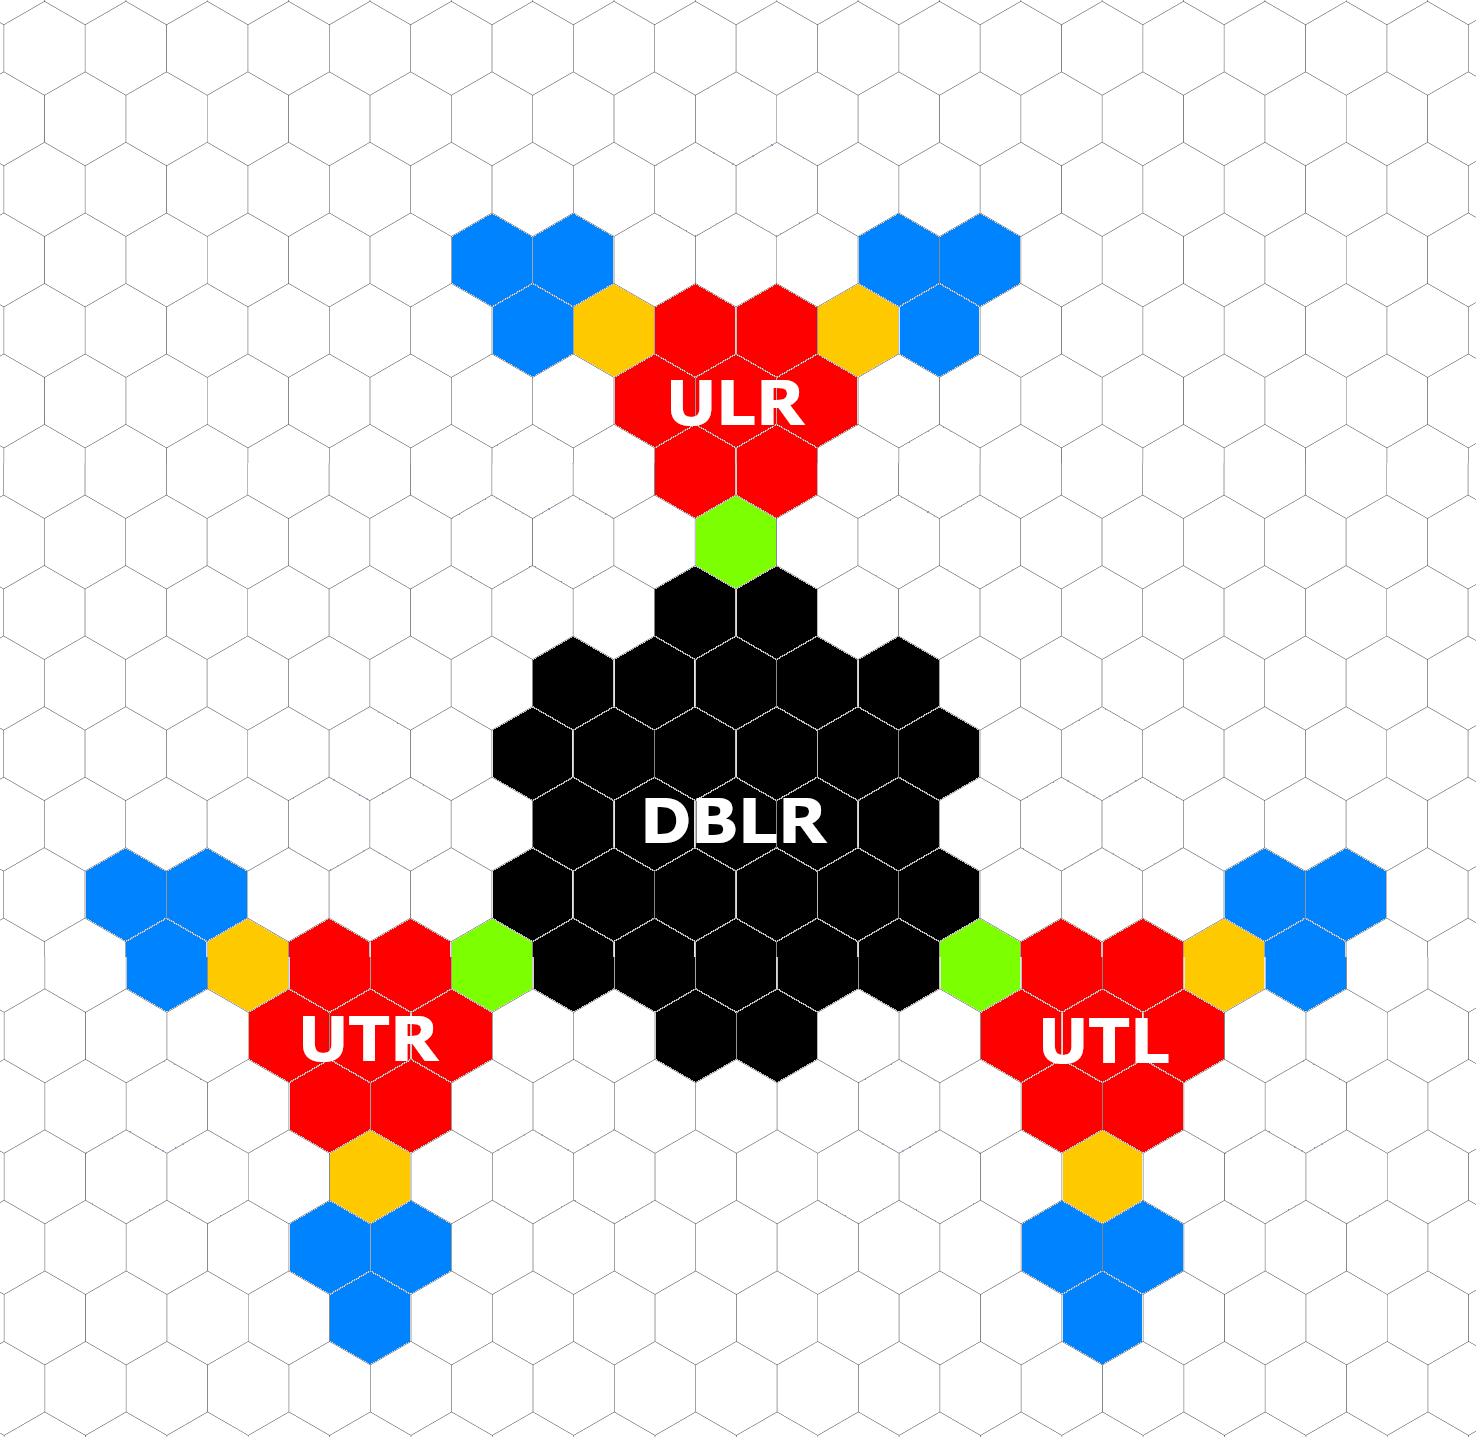
\includegraphics[width=0.45\linewidth]{img/Aethereu/UTLR.png}
	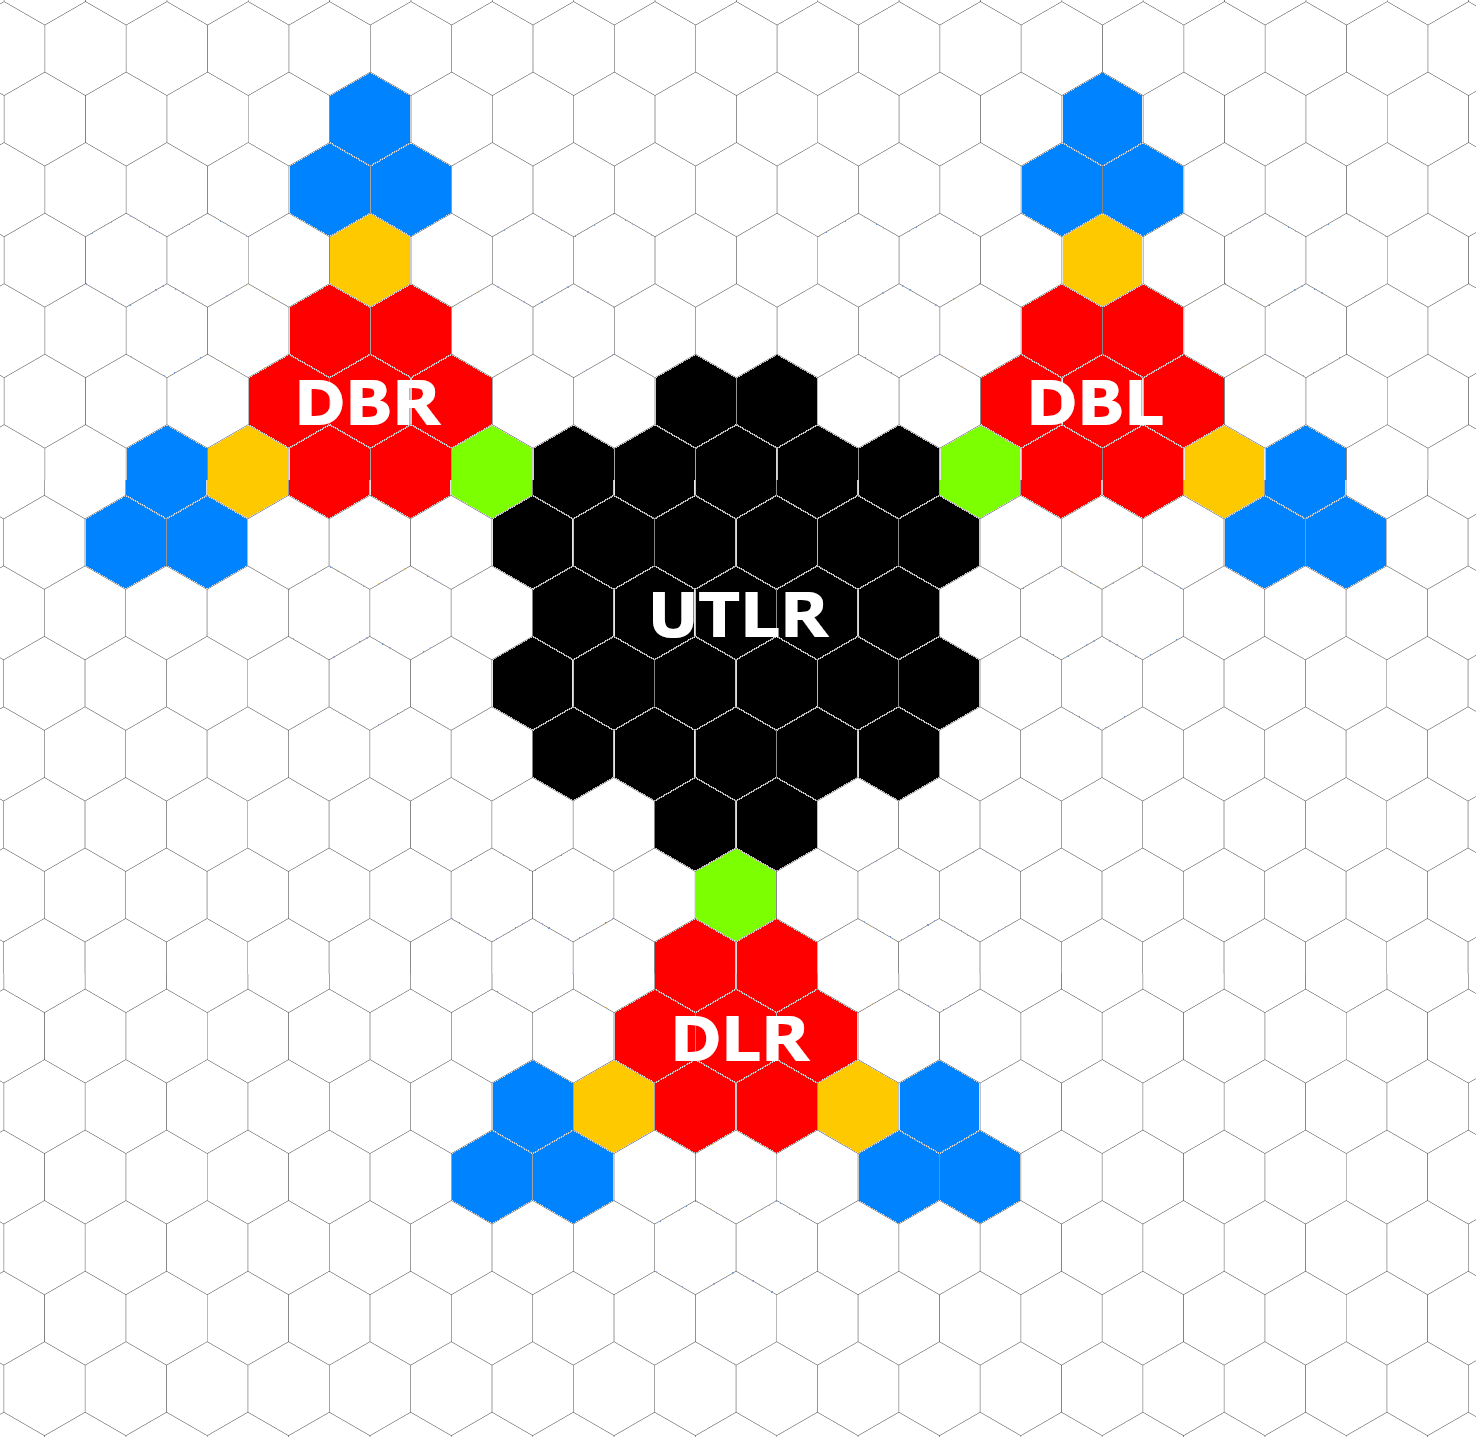
\includegraphics[width=0.45\linewidth]{img/Aethereu/DBLR.png}
		
	\textbf{UTLR} \hspace{7cm} \textbf{DBLR}
\end{center}

The labels on the different chamber configurations are labels for how they are oriented. These follow as
\begin{dndtable}[cX]
	\textbf{Label} & \textbf{Meaning} \\
	U           & Up Facing Triangle\\
	D           & Down Facing Triangle \\
	L           & Left Room Turned \\
	R           & Right Room Turned \\
	T           & Top Room Turned\\
	B           & Bottom Room Turned \\
\end{dndtable}



To successfully navigate through the chamber the party must move around such that the rooms are in the \textbf{U} configuration. If done properly, a pedestal will arise from the center chamber containing the space stone. The pedestal will be slightly off centered towards the peak of the triangle. If the party attempts to grab the stone in this state, they will be slowly torn from reality and returned to when they entered The Pluvian Forest (backwards in time). As this is happening, Nev\'{a}r will appear and give a spiel about how they helped her free her pet. Then, after being torn from the moment, they will be taken through time to a vision of a great beast/demon being captured in the energy stone (an un-recorded piece of lore per-say). As a penalty of the un-seen energy stone, a great demon lord will have arrived at the location of Aethereu destroying it and summoning creatures from other dimensional realms (void creatures, demonic creatures, and beast creatures).

Throughout the time in Aethereu, there will be occasional glimpses through and ahead of time. This can be party member images entering a specific door, or party member images calling out something. The flow of time wants to be preserved and the party must act out these that they see as they see them so that there are no inconsistencies in the temporal flow. If done correctly, then once the configuration of the rooms is correct, two pedestals will appear instead of one. The second to the left of the first, forming sort of half a tri-force. This second pedestal will contain the time stone. If the party attempts to grab the stone(s) in this state, the same effect described above will happen due to the energy stone, but not the time stone.
